%%%%%%%%%%%%%%%%%%%%%%%%%%%%%%%%%%%%%%%%%
% Masters/Doctoral Thesis 
% LaTeX Template
% Version 2.2 (21/11/15)
%
% This template has been downloaded from:
% http://www.LaTeXTemplates.com
%
% Version 2.x major modifications by:
% Vel (vel@latextemplates.com)
%
% This template is based on a template by:
% Steve Gunn (http://users.ecs.soton.ac.uk/srg/softwaretools/document/templates/)
% Sunil Patel (http://www.sunilpatel.co.uk/thesis-template/)
%
% Template license:
% CC BY-NC-SA 3.0 (http://creativecommons.org/licenses/by-nc-sa/3.0/)
%
%%%%%%%%%%%%%%%%%%%%%%%%%%%%%%%%%%%%%%%%%

%----------------------------------------------------------------------------------------
%	PACKAGES AND OTHER DOCUMENT CONFIGURATIONS
%----------------------------------------------------------------------------------------

\documentclass[
11pt, % The default document font size, options: 10pt, 11pt, 12pt
oneside, % Two side (alternating margins) for binding by default, uncomment to switch to one side
english, % ngerman for German
singlespacing, % Single line spacing, alternatives: onehalfspacing or doublespacing
%draft, % Uncomment to enable draft mode (no pictures, no links, overfull hboxes indicated)
%nolistspacing, % If the document is onehalfspacing or doublespacing, uncomment this to set spacing in lists to single
%liststotoc, % Uncomment to add the list of figures/tables/etc to the table of contents
%toctotoc, % Uncomment to add the main table of contents to the table of contents
%parskip, % Uncomment to add space between paragraphs
%nohyperref, % Uncomment to not load the hyperref package
headsepline, % Uncomment to get a line under the header
]{MastersDoctoralThesis} % The class file specifying the document structure

\usepackage[UTF8, heading = false, scheme = plain]{ctex}

\usepackage[utf8]{inputenc} % Required for inputting international characters
\usepackage[T1]{fontenc} % Output font encoding for international characters
\usepackage{palatino} % Use the Palatino font by default


\usepackage[backend=bibtex,style=authoryear,natbib=true]{biblatex} % User the bibtex backend with the authoryear citation style (which resembles APA)

\addbibresource{example.bib} % The filename of the bibliography

\usepackage[autostyle=true]{csquotes} % Required to generate language-dependent quotes in the bibliography

\usepackage{float}
\usepackage{tabu}

\usepackage{indentfirst}
\setlength{\parindent}{2em}
\setlength{\parskip}{7pt}
\linespread{1.2}

%----------------------------------------------------------------------------------------
%	MARGIN SETTINGS
%----------------------------------------------------------------------------------------

\geometry{
	paper=a4paper, % Change to letterpaper for US letter
	inner=3.5cm, % Inner margin
	outer=3.5cm, % Outer margin
	%bindingoffset=2cm, % Binding offset
	top=2cm, % Top margin
	bottom=2cm, % Bottom margin
	%showframe,% show how the type block is set on the page
}

%----------------------------------------------------------------------------------------
%	THESIS INFORMATION
%----------------------------------------------------------------------------------------

\thesistitle{计算机实验报告} % Your thesis title, this is used in the title and abstract, print it elsewhere with \ttitle
\supervisor{刘卫东、李山山} % Your supervisor's name, this is used in the title page, print it elsewhere with \supname
\examiner{} % Your examiner's name, this is not currently used anywhere in the template, print it elsewhere with \examname
\degree{} % Your degree name, this is used in the title page and abstract, print it elsewhere with \degreename
\author{董胤蓬、钱雨杰、桥本优} % Your name, this is used in the title page and abstract, print it elsewhere with \authorname
\addresses{} % Your address, this is not currently used anywhere in the template, print it elsewhere with \addressname

\subject{Computer Sciences and Technology} % Your subject area, this is not currently used anywhere in the template, print it elsewhere with \subjectname
\keywords{} % Keywords for your thesis, this is not currently used anywhere in the template, print it elsewhere with \keywordnames
\university{\href{http://www.tsinghua.edu.cn}{清华大学}} % Your university's name and URL, this is used in the title page and abstract, print it elsewhere with \univname
\department{\href{http://department.university.com}{计算机科学与技术系}} % Your department's name and URL, this is used in the title page and abstract, print it elsewhere with \deptname
\group{\href{http://researchgroup.university.com}{Research Group Name}} % Your research group's name and URL, this is used in the title page, print it elsewhere with \groupname
\faculty{\href{http://faculty.university.com}{Faculty Name}} % Your faculty's name and URL, this is used in the title page and abstract, print it elsewhere with \facname

\hypersetup{pdftitle=\ttitle} % Set the PDF's title to your title
\hypersetup{pdfauthor=\authorname} % Set the PDF's author to your name
\hypersetup{pdfkeywords=\keywordnames} % Set the PDF's keywords to your keywords

\begin{document}

\frontmatter % Use roman page numbering style (i, ii, iii, iv...) for the pre-content pages

\pagestyle{plain} % Default to the plain heading style until the thesis style is called for the body content

%----------------------------------------------------------------------------------------
%	TITLE PAGE
%----------------------------------------------------------------------------------------

\begin{titlepage}
\begin{center}

\includegraphics[width=0.3\textwidth]{Figures/thu.png}\\[1cm]
\textsc{\LARGE \univname}\\[0.8cm] % University name
\textsc{\LARGE 计算机组成原理}\\[0.5 cm] % Thesis type

\HRule \\[0.4cm] % Horizontal line
{\huge \bfseries \ttitle}\\[0.4cm] % Thesis title
\large \textit{支持THCO MIPS指令系统的流水线计算机设计与实现}\\[0.3cm] % University requirement text
\HRule \\[1.5cm] % Horizontal line
 
\begin{minipage}{0.4\textwidth}
\begin{flushleft} \large
\emph{作者:}\\[0.4cm] 
\authorname % Author name - remove the \href bracket to remove the link
\end{flushleft}
\end{minipage}
\begin{minipage}{0.4\textwidth}
\begin{flushright} \large
\emph{指导教师:} \\[0.4cm]
\supname % Supervisor name - remove the \href bracket to remove the link  
\end{flushright}
\end{minipage}\\[4cm]

%\textit{in the}\\[0.4cm]
\univname\\[0.1cm]\deptname\\[2cm] % Research group name and department name
 
{\large \today}\\[3cm] % Date
%\includegraphics{Logo} % University/department logo - uncomment to place it
 
\vfill
\end{center}
\end{titlepage}

%----------------------------------------------------------------------------------------
%	ABSTRACT PAGE
%----------------------------------------------------------------------------------------

\begin{abstract}
\addchaptertocentry{\abstractname} % Add the abstract to the table of contents

The Thesis Abstract is written here (and usually kept to just this page). The page is kept centered vertically so can expand into the blank space above the title too\ldots

\end{abstract}

%----------------------------------------------------------------------------------------
%	LIST OF CONTENTS/FIGURES/TABLES PAGES
%----------------------------------------------------------------------------------------

\tableofcontents % Prints the main table of contents

%\listoffigures % Prints the list of figures

%\listoftables % Prints the list of tables


%----------------------------------------------------------------------------------------
%	THESIS CONTENT - CHAPTERS
%----------------------------------------------------------------------------------------

\mainmatter % Begin numeric (1,2,3...) page numbering

\pagestyle{thesis} % Return the page headers back to the "thesis" style

% Include the chapters of the thesis as separate files from the Chapters folder
% Uncomment the lines as you write the chapters

% Chapter 1

\chapter{实验目的} % Main chapter title

\label{Chapter1} % For referencing the chapter elsewhere, use \ref{Chapter1} 

%----------------------------------------------------------------------------------------

% Define some commands to keep the formatting separated from the content 
\newcommand{\keyword}[1]{\textbf{#1}}
\newcommand{\tabhead}[1]{\textbf{#1}}
\newcommand{\code}[1]{\texttt{#1}}
\newcommand{\file}[1]{\texttt{\bfseries#1}}
\newcommand{\option}[1]{\texttt{\itshape#1}}

本实验是清华大学计算机科学与技术系开设的《计算机组成原理》课程实验。

实验任务是设计和实现一台16位支持指令流水的计算机。实验计算机的CPU采用五段流水线结构,支持THCO MIPS指令系统,并适当应用数据旁路、分支预测等技术提高流水线效率;使用SRAM作为存储器,并对内存进行管理;实验计算机的I/O通过串口与运行终端程序的PC连接,实现输入输出。实验计算机实现后需要运行监控程序,并可以通过监控程序实现用户写入指令、执行指令、查看寄存器和内存等操作。

实验可以在基础要求上进行一些扩展,包括软硬件中断处理、PS2键盘输入、VGA输出、双机通信、多道程序等。

通过实验,可以加深对于计算机系统知识的理解,进一步理解和掌握流水线结构计算机的各部件组成和内部工作原理,掌握计算机外部设备输入输出的设计实现,培养硬件设计和调试的能力。

%----------------------------------------------------------------------------------------


% Chapter Template

\chapter{实验环境} % Main chapter title

\label{Chapter2} % Change X to a consecutive number; for referencing this chapter elsewhere, use \ref{ChapterX}

%----------------------------------------------------------------------------------------
%	SECTION 1
%----------------------------------------------------------------------------------------

\section{硬件环境}

Lorem ipsum dolor sit amet, consectetur adipiscing elit. Aliquam ultricies lacinia euismod. Nam tempus risus in dolor rhoncus in interdum enim tincidunt. Donec vel nunc neque. In condimentum ullamcorper quam non consequat. Fusce sagittis tempor feugiat. Fusce magna erat, molestie eu convallis ut, tempus sed arcu. Quisque molestie, ante a tincidunt ullamcorper, sapien enim dignissim lacus, in semper nibh erat lobortis purus. Integer dapibus ligula ac risus convallis pellentesque.

%-----------------------------------
%	SUBSECTION 1
%-----------------------------------
\subsection{Subsection 1}

Nunc posuere quam at lectus tristique eu ultrices augue venenatis. Vestibulum ante ipsum primis in faucibus orci luctus et ultrices posuere cubilia Curae; Aliquam erat volutpat. Vivamus sodales tortor eget quam adipiscing in vulputate ante ullamcorper. Sed eros ante, lacinia et sollicitudin et, aliquam sit amet augue. In hac habitasse platea dictumst.

%-----------------------------------
%	SUBSECTION 2
%-----------------------------------

\subsection{Subsection 2}
Morbi rutrum odio eget arcu adipiscing sodales. Aenean et purus a est pulvinar pellentesque. Cras in elit neque, quis varius elit. Phasellus fringilla, nibh eu tempus venenatis, dolor elit posuere quam, quis adipiscing urna leo nec orci. Sed nec nulla auctor odio aliquet consequat. Ut nec nulla in ante ullamcorper aliquam at sed dolor. Phasellus fermentum magna in augue gravida cursus. Cras sed pretium lorem. Pellentesque eget ornare odio. Proin accumsan, massa viverra cursus pharetra, ipsum nisi lobortis velit, a malesuada dolor lorem eu neque.

%----------------------------------------------------------------------------------------
%	SECTION 2
%----------------------------------------------------------------------------------------

\section{软件环境}

Sed ullamcorper quam eu nisl interdum at interdum enim egestas. Aliquam placerat justo sed lectus lobortis ut porta nisl porttitor. Vestibulum mi dolor, lacinia molestie gravida at, tempus vitae ligula. Donec eget quam sapien, in viverra eros. Donec pellentesque justo a massa fringilla non vestibulum metus vestibulum. Vestibulum in orci quis felis tempor lacinia. Vivamus ornare ultrices facilisis. Ut hendrerit volutpat vulputate. Morbi condimentum venenatis augue, id porta ipsum vulputate in. Curabitur luctus tempus justo. Vestibulum risus lectus, adipiscing nec condimentum quis, condimentum nec nisl. Aliquam dictum sagittis velit sed iaculis. Morbi tristique augue sit amet nulla pulvinar id facilisis ligula mollis. Nam elit libero, tincidunt ut aliquam at, molestie in quam. Aenean rhoncus vehicula hendrerit. 
% Chapter Template

\chapter{实验设计} % Main chapter title

\label{Chapter3} % Change X to a consecutive number; for referencing this chapter elsewhere, use \ref{ChapterX}

%----------------------------------------------------------------------------------------
%	SECTION 1
%----------------------------------------------------------------------------------------

\section{CPU流水结构}


%-----------------------------------
%	SUBSECTION 1
%-----------------------------------
\subsection{整体设计}


我们设计并实现了五级流水结构的CPU,对每条指令的处理分为IF、ID、EXE、MEM、WB五个阶段。采用25M时钟,每个时钟周期流水线的每一个阶段完成一条指令的一部分,不同阶段并行完成不同指令的不同部分。同时每两个阶段之间均有一个段间锁存器,用与接收上一阶段的信号并在下一个时钟上升沿到来时传递到下一阶段。

流水线五个阶段的功能与所占用的资源如下:

IF:根据输入的PC值从内存中取出指令。在执行写入命令时,还需要根据PC值向内存中写入用户指令。占用资源:IM、PC、总线

ID:根据IF阶段读取的指令进行译码,从寄存器堆中读出所需寄存器的值。占用资源:寄存器组

EXE:根据ID阶段生成的控制信号、操作数和操作符进行计算,将结果传递到下一阶段。占用资源:ALU

MEM:根据ID阶段生成的控制信号执行写入内存和读取内存的操作,在实现时还需考虑串口的读写与VGA/Keyboard的读写访问。占用资源:DM、总线

WB:根据控制信号执行写回寄存器的操作。占用资源:寄存器组

%-----------------------------------
%	SUBSECTION 2
%-----------------------------------

\subsection{数据通路}

我们设计的数据通路见Figure 3.1.
\begin{figure}[H]
  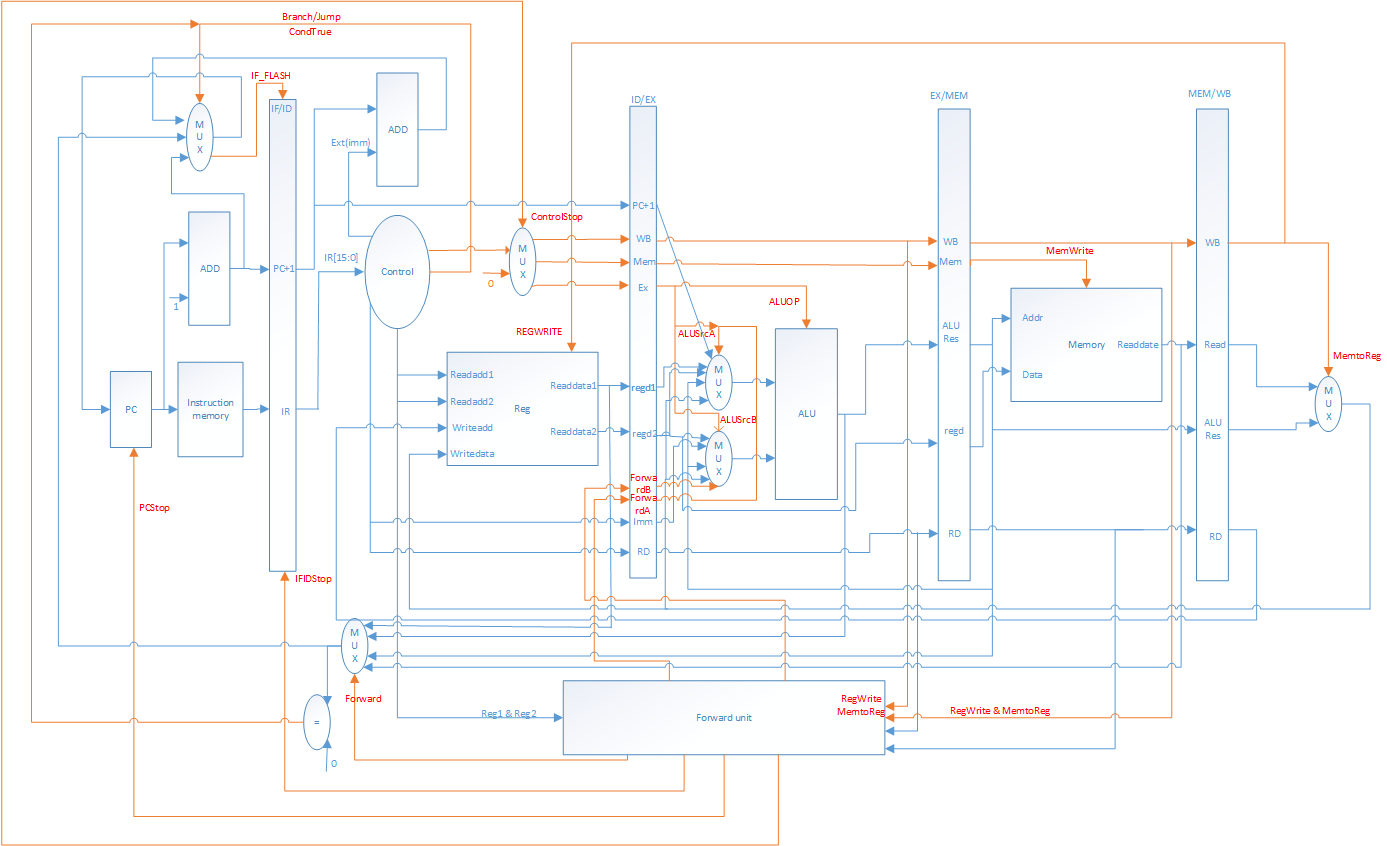
\includegraphics[width=\linewidth]{Figures/datapath.png}
  \caption{数据通路.}
\end{figure}

在数据通路的设计上,我们基本遵循经典的五级流水线结构,但是在其基础之上有了一些变化和改进。

我们将处理数据冲突的模块全部放在了Forward Unit中。既可以将在EXE、MEM的计算结果流回到下一条指令的EXE阶段,同时也可以对访存操作的数据冲突进行插气泡处理。Forward Unit模块还可以处理跳转指令的数据冲突,这样整体结构更加简洁。

我们新增PC模块,同于计算下一周期取指的PC值,根据跳转信号进行计算,可以解决控制冲突。具体实现见冲突处理部分。

%-----------------------------------
%	SUBSECTION 3
%-----------------------------------

\subsection{控制信号}
在ID阶段译码的过程中,会产生很多控制信号,针对我们所需实现的30条指令的指令集,我们设计的控制信号为:

ALUOP:ALU运算器的操作符,包括的类型有 ADD(加法)、SUB(减法)、ASSIGNA(赋操作数A的值)、ASSIGNB(赋操作数B的值)、AND(与)、OR(或)、SLL(逻辑左移)、SRA(算数右移)、EQUAL(判断相等)、LESS(判断小于)、EMPTY(无操作)。

SRCREGA:读取第一个寄存器值的控制使能。1表示IR[10:8],0表示特殊寄存器。

SRCREGB:读取第二个寄存器值的控制使能。1表示IR[10:8],0表示IR[7:5]。

REGDST:写回寄存器编号的控制使能。00表示特殊寄存器,01表示IR[10:8],10表示IR[7:5],11表示IR[4:2]。

ALUSRCA:ALU运算器第一个操作数的选择信号。00表示Reg[IR[10:8]],01表示Reg[IR[7:5]],10表示EPC。

ALUSRCB:ALU运算器第二个操作数的选择信号。1表示reg[IR[7:5]],0表示extend(imm)。

EXTOP:立即数扩展方式。0表示符号扩展,1表示零扩展。

MEMTOREG:读取内存并写回寄存器使能。

REGWRITE:写回寄存器使能。

MEMWRITE:内存写使能。

BRANCH:B指令跳转信号。00表示无B型跳转,10表示无条件跳转,01表示不等条件跳转,11表示相等条件跳转。

JUMP:J指令跳转使能。

对于每条指令的控制信号,见表3.1—3.5,其中的‘x’表示没有使用。

\begin{table}[H]
\begin{center}
\renewcommand{\arraystretch}{1.3}
\small
\caption{Control Signals}
\label{tab:treatments}
\begin{tabular}{|>{\centering}p{2.1cm}|*{6}{p{1.4cm}<{\centering}}|}
\hline
& ADDIU & ADDIU3 & ADDSP & ADDU & AND & B \\
\hline
ALUOP & ADD	& ADD & ADD & ADD & AND & EMPTY\\	
\hline
SRCREGA & 1 & 1 & 0 & 1 & 1 & x\\
\hline
SRCREGB & x & x & x & 0 & 0 & x\\
\hline
REGDST & 01 & 10 & 00 & 11 & 01 & x\\
\hline
ALUSRCA & 00 & 00 & 00 & 00 & 00 & x\\
\hline
ALUSRCB & 0 & 0 & 0 & 1 & 1 & x\\
\hline
EXTOP & 0 & 0 & 0 & x & x & 0\\
\hline
MEMTOREG & 0 & 0 & 0 & 0 & 0 & 0\\
\hline
REGWRITE & 1 & 1 & 1 & 1 & 1 & 0\\
\hline
MEMWRITE & 0 & 0 & 0 & 0 & 0 & 0\\
\hline
BRANCH & 00 & 00 & 00 & 00 & 00 & 10\\
\hline
JUMP & 0 & 0 & 0 & 0 & 0 & 0\\
\hline
\end{tabular}
\end{center}
\end{table}


\begin{table}[H]
\begin{center}
\renewcommand{\arraystretch}{1.3}
\small
\caption{Control Signals}
\label{tab:treatments}
\begin{tabular}{|>{\centering}p{2.1cm}|*{6}{p{1.4cm}<{\centering}}|}
\hline
& BEQZ & BNEZ & BTEQZ & CMP & CMPI & JALR \\
\hline
ALUOP & EMPTY & EMPTY & EMPTY & EQUAL & EQUAL & ASSIGNA\\	
\hline
SRCREGA & 1 & 1 & 0 & 1 & 1 & 1\\
\hline
SRCREGB & x & x & x & 0 & x & x\\
\hline
REGDST & x & x & x & 00 & 00 & 00\\
\hline
ALUSRCA & x & x & x & 00 & 00 & 10\\
\hline
ALUSRCB & x & x & x & 1 & 0 & x\\
\hline
EXTOP & 0 & 0 & 0 & x & 0 & x\\
\hline
MEMTOREG & 0 & 0 & 0 & 0 & 0 & 0\\
\hline
REGWRITE & 0 & 0 & 0 & 1 & 1 & 1\\
\hline
MEMWRITE & 0 & 0 & 0 & 0 & 0 & 0\\
\hline
BRANCH & 11 & 01 & 11 & 00 & 00 & 00\\
\hline
JUMP & 0 & 0 & 0 & 0 & 0 & 1\\
\hline
\end{tabular}
\end{center}
\end{table}


\begin{table}[H]
\begin{center}
\renewcommand{\arraystretch}{1.3}
\small
\caption{Control Signals}
\label{tab:treatments}
\begin{tabular}{|>{\centering}p{2.1cm}|*{6}{p{1.4cm}<{\centering}}|}
\hline
& JR & JRRA & LI & LW & LW$\_$SP & MFIH \\
\hline
ALUOP & EMPTY & EMPTY & ASSIGNB & ADD & ADD & ASSIGNA\\	
\hline
SRCREGA & 1 & 0 & x & 1 & 0 & 0\\
\hline
SRCREGB & x & x & x & x & x & x\\
\hline
REGDST & x & x & 01 & 10 & 01 & 01\\
\hline
ALUSRCA & x & x & x & 00 & 00 & 00\\
\hline
ALUSRCB & x & x & 0 & 0 & 0 & x\\
\hline
EXTOP & x & x & 1 & 0 & 0 & x\\
\hline
MEMTOREG & 0 & 0 & 0 & 1 & 1 & 0\\
\hline
REGWRITE & 0 & 0 & 1 & 1 & 1 & 1\\
\hline
MEMWRITE & 0 & 0 & 0 & 0 & 0 & 0\\
\hline
BRANCH & 00 & 00 & 00 & 00 & 00 & 00\\
\hline
JUMP & 1 & 1 & 0 & 0 & 0 & 0\\
\hline
\end{tabular}
\end{center}
\end{table}


\begin{table}[H]
\begin{center}
\renewcommand{\arraystretch}{1.3}
\small
\caption{Control Signals}
\label{tab:treatments}
\begin{tabular}{|>{\centering}p{2.1cm}|*{6}{p{1.4cm}<{\centering}}|}
\hline
& MFPC & MOVE & MTIH & MTSP & NOP & OR \\
\hline
ALUOP & ASSIGNA & ASSIGNA & ASSIGNA & ASSIGNA & EMPTY & OR\\	
\hline
SRCREGA & x & x & 1 & x & x & 1\\
\hline
SRCREGB & x & 0 & x & 0 & x & 0\\
\hline
REGDST & 01 & 01 & 00 & 00 & x & 01\\
\hline
ALUSRCA & 10 & 01 & 00 & 01 & x & 00\\
\hline
ALUSRCB & x & x & x & x & x & 1\\
\hline
EXTOP & x & x & x & x & x & x\\
\hline
MEMTOREG & 0 & 0 & 0 & 0 & 0 & 0\\
\hline
REGWRITE & 1 & 1 & 1 & 1 & 0 & 1\\
\hline
MEMWRITE & 0 & 0 & 0 & 0 & 0 & 0\\
\hline
BRANCH & 00 & 00 & 00 & 00 & 00 & 00\\
\hline
JUMP & 0 & 0 & 0 & 0 & 0 & 0\\
\hline
\end{tabular}
\end{center}
\end{table}


\begin{table}[H]
\begin{center}
\renewcommand{\arraystretch}{1.3}
\small
\caption{Control Signals}
\label{tab:treatments}
\begin{tabular}{|>{\centering}p{2.1cm}|*{6}{p{1.4cm}<{\centering}}|}
\hline
& SLL & SLTI & SRA & SUBU & SW & SW$\_$SP \\
\hline
ALUOP & SLL & LESS & SRA & SUB & ADD & ADD\\	
\hline
SRCREGA & x & 1 & x & 1 & 1 & 0\\
\hline
SRCREGB & 0 & x & 0 & 0 & 0 & 1\\
\hline
REGDST & 01 & 00 & 01 & 11 & x & x\\
\hline
ALUSRCA & 01 & 00 & 01 & 00 & 00 & 00\\
\hline
ALUSRCB & 0 & 0 & 0 & 1 & 0 & 0\\
\hline
EXTOP & 1 & 0 & 1 & x & 0 & 0\\
\hline
MEMTOREG & 0 & 0 & 0 & 0 & 0 & 0\\
\hline
REGWRITE & 1 & 1 & 1 & 1 & 0 & 0\\
\hline
MEMWRITE & 0 & 0 & 0 & 0 & 1 & 1\\
\hline
BRANCH & 00 & 00 & 00 & 00 & 00 & 00\\
\hline
JUMP & 0 & 0 & 0 & 0 & 0 & 0\\
\hline
\end{tabular}
\end{center}
\end{table}

除了以上通过译码器产生的控制信号外,还有FORWARD UNIT产生的冲突处理信号,我们将在下一节详细说明。
%-----------------------------------
%	SUBSECTION 4
%-----------------------------------

\subsection{冲突处理}
\subsubsection{结构冲突}
我们采用指令与数据分离存储的方式来避免结构冲突问题。用RAM1和RAM2分别存储数据和指令。但在监控程序功能中有一个 A 指令需要向指令存储器中写入用户指令,这时,我们通过在MEM阶段判断写入地址是否为指令内存地址区间,并产生控制信号IFWE。在IF阶段如果接收到信号IFWE,则将流水线暂停一个周期用来写入指令。

\subsubsection{数据冲突}
我们在这里仅讨论两种不涉及跳转的数据冲突,两种冲突分别为涉及访存和不涉及访存的冲突。比如:

\textbf{\textit{Example1}}: \quad ADDU R1 R2 R3; \quad SLL R3 R3 0x00

\textbf{\textit{Example2}}: \quad LW R1 R3 0x00; \quad SLL R3 R3 0x00

数据冲突产生原因是前一条指令或者前两条指令需要写回寄存器,而当前的指令又要访问寄存器中的值。这时我们通过增加旁路的方式将之前的计算结果传输到当前的操作数上。

在FORWARD UNIT中,通过判断上一条指令(或上两条指令)的写回寄存器编号与当前目的寄存器编号是否相等来判断是否发生数据冲突。对于涉及访存的数据冲突,我们需要插入气泡等待一个周期,使得上一条指令MEM阶段执行完毕取出内存数之后,再参与下一条指令的运算。FORWARD UNIT产生的控制信号为:

FORWARDA:ALU第一个操作数选择信号。00表示无冲突,使用ID阶段读取的寄存器的值;01表示与上一条指令发生冲突,选择ALU的结果;10表示与上两条指令发生冲突,选择MEM的结果

FORWARDB:ALU第二个操作数选择信号。与FORWARDA类似。

PCSTOP,IFIDSTOP,CONTROLSTOP:插入气泡的控制信号。

\subsubsection{控制冲突}

控制冲突是由于B指令与J指令而产生的。我们将跳转地址的计算放在ID阶段执行。这样,在控制器译码结束后,可以直接计算出跳转后的PC值,故这种做法不需要分支预测,可以提高速度。另外,我们采用打开延迟槽的策略,对跳转指令的后一条指令继续执行。

在实际的冲突中,控制冲突往往与数据冲突结合在一起,比如:

\textbf{\textit{Example3}}: \quad ADDU R1 R2 R3; \quad JR R3;

\textbf{\textit{Example4}}: \quad LW R1 R3 0x00; \quad BEQZ R3 0x10;

在以上的两个例子中,既发生了控制冲突,同时也存在数据冲突。我们同样使用增加旁路的办法,唯一的不同在于旁路的信号需要传送到ID阶段进行计算。FORWARD UNIT模块同样可以产生数据冲突的信号,用于选择跳转所需的寄存器的值。在PC模块中,根据跳转信号与冲突选择信号选取下一条指令的PC值。

%----------------------------------------------------------------------------------------
%	SECTION 2
%----------------------------------------------------------------------------------------

\section{寄存器堆}

寄存器堆用于存放所有寄存器的值,用于在ID阶段读取寄存器值与WB阶段写回寄存器的值。读寄存器值为组合逻辑,在信号稳定之前读取的值被锁在ID$\_$EXE段间的锁存器中,故不会对后面的结果产生影响。写寄存器值为时序逻辑,必须等待信号稳定后才能写回。由于MEM$\_$WB段间锁存器在上升沿触发,故在下降沿进行写回,此时信号已经稳定。

我们将R0-R7这八个通用寄存器放在寄存器堆中,同时还将SP、RA、IH、T四个系统寄存器也放在寄存器堆中,以方便处理。这样,寄存器的编号需要从三位扩展为四位。各寄存器的编号见表3.6.

\begin{table}[H]
\begin{center}
\renewcommand{\arraystretch}{1.3}
\small
\caption{Register Cluster}
\label{tab:treatments}
\begin{tabular}{|p{1.4cm}<{\centering}|p{3cm}<{\centering}|p{1.4cm}<{\centering}|}
\hline
符号 & 含义 & 编号 \\
\hline
R0 & 通用寄存器 & 0000 \\
\hline
R1 & 通用寄存器 & 0001 \\
\hline
R2 & 通用寄存器 & 0010 \\
\hline
R3 & 通用寄存器 & 0011 \\
\hline
R4 & 通用寄存器 & 0100 \\
\hline
R5 & 通用寄存器 & 0101 \\
\hline
R6 & 通用寄存器 & 0110 \\
\hline
R7 & 通用寄存器 & 0111 \\
\hline
SP & 栈顶指针寄存器 & 1001 \\
\hline
T & T标志寄存器 & 1010 \\
\hline
IH & 中断寄存器 & 1011 \\
\hline 
RA & 返回值寄存器 & 1100 \\
\hline
\end{tabular}
\end{center}
\end{table}


%----------------------------------------------------------------------------------------
%	SECTION 3
%----------------------------------------------------------------------------------------

\section{存储器}

%----------------------------------------------------------------------------------------
%	SECTION 4
%----------------------------------------------------------------------------------------

\section{中断处理}

我们实现了四种类型的中断,其中包括两种硬件中断(ESC中断:返回到中断PC;Control C中断:返回到监控程序),软件中断,时钟中断。下面对这四种中断分别介绍。

\subsection{ESC硬件中断}

ESC硬件中断是通过在用户程序执行时,键盘摁下ESC键产生的中断,在监控程序执行时无效。ESC中断发生时,调用中断处理程序输出中断号,并返回到发生中断的指令继续执行。

这部分硬件中断会复用监控程序的delint中断处理代码,在中断处理程序中需要用到中断时的PC以及中断号,所以需要在发生中断时通过硬件来保存PC与中断号,并跳到中断处理程序。在IF$\_$ID的段间锁存器中加入状态机,来处理ESC中断。状态机见Figure 3.2.

\begin{figure}[H]
  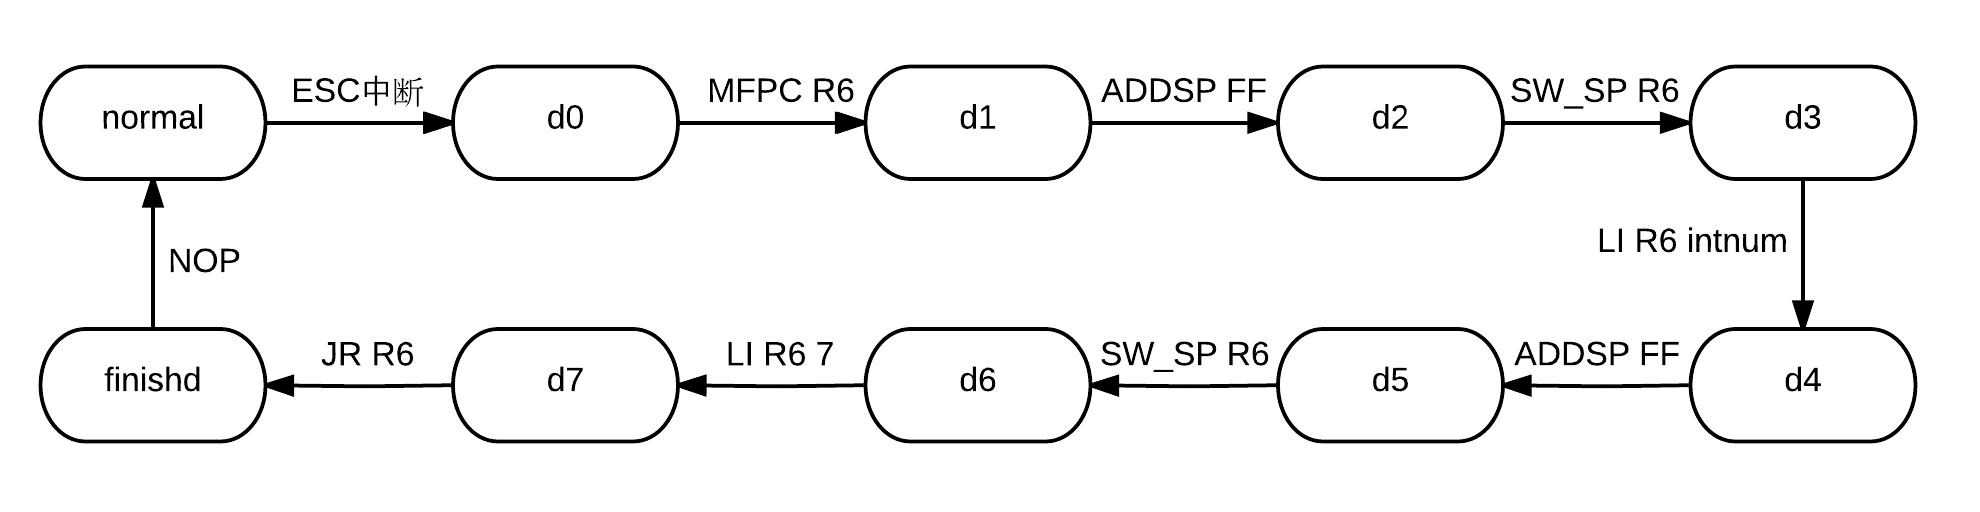
\includegraphics[width=\linewidth]{Figures/escint.png}
  \caption{ESC硬件中断状态机.}
\end{figure}

其中箭头上的指令为每个状态机下输出的指令,用来向栈中存储PC值和中断号。保存完毕后,跳到中断处理程序执行,同时状态回到normal。

\subsection{Control C硬件中断}

ESC硬件中断的不足在于对于死循环的用户程序,中断发生后无法跳出死循环,而是继续回到中断发生的位置执行。我们希望仿照真正计算机上的Control C功能,可以实现跳出用户程序的功能。

Control C中断的处理与ESC硬件中断类似,但是不需要再次返回中断时的PC,而是直接跳到监控程序的BEGIN部分即可。所以处理过程比ESC更加简单,只需要在中断发生后将中断号入栈即可,不需要保存PC值。同时需要在监控程序中加入Control C中断的处理。状态机见Figure 3.3.

\begin{figure}[H]
  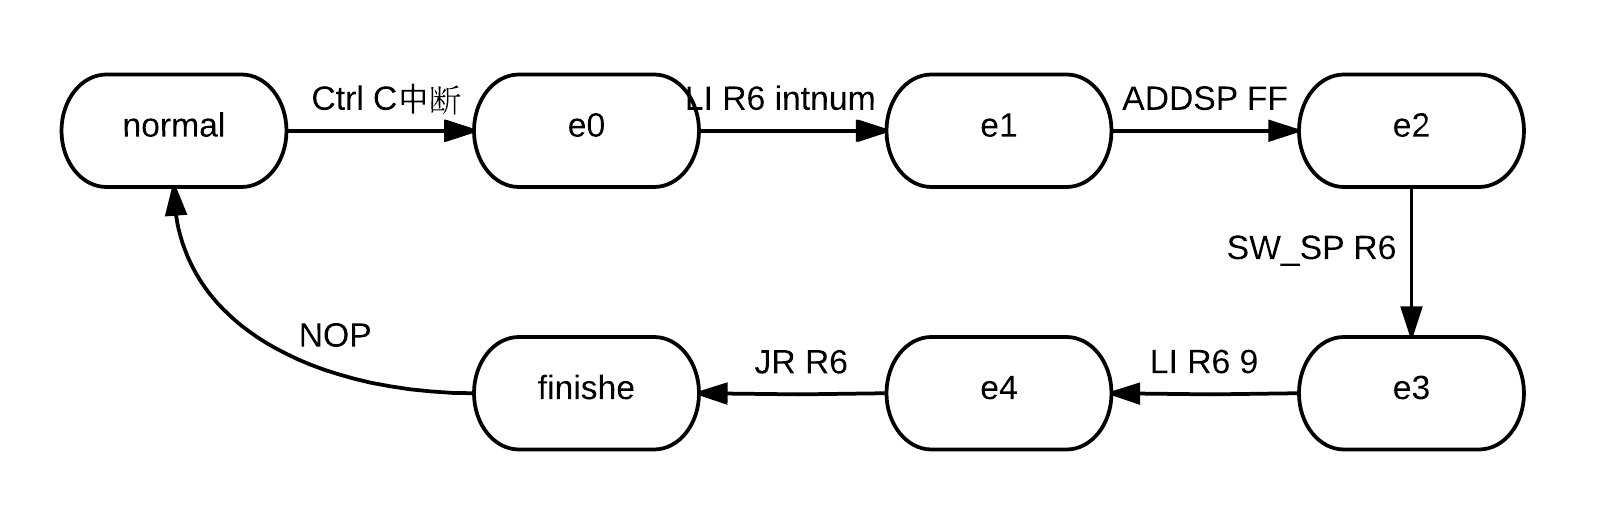
\includegraphics[width=\linewidth]{Figures/ctrl_c.png}
  \caption{Control C硬件中断状态机.}
\end{figure}

\subsection{软件中断}

软件中断的原理与ESC硬件中断一样,通过在控制器译码时产生软件中断的信号,传到IF$\_$ID段间锁存器,同时将软件中断号同时传回,按照ESC的状态机处理软件中断。

\subsection{时钟中断}

时钟中断指计时时钟到一定的时间后,产生中断信号。我们做时钟中断的原因是为了之后的多道程序,多道程序需要分时执行两套监控程序,故需要有分时机制。多道程序的细节在后面讨论,这里仅讨论一下时钟中断的处理。

时钟中断的处理过程与ESC硬件中断基本一致,但是需要注意的一个地方是ESC硬件中断只会发生在用户程序中,这时我们就可以随意使用R6、R7的值(因为用户程序不允许使用)。但是时钟中断可以发生在任何地方,在执行监控程序时也会有时钟中断,所以要首先保存R6的值,才可以执行后续的保存现场的指令。状态机见Figure 3.4.

\begin{figure}[H]
  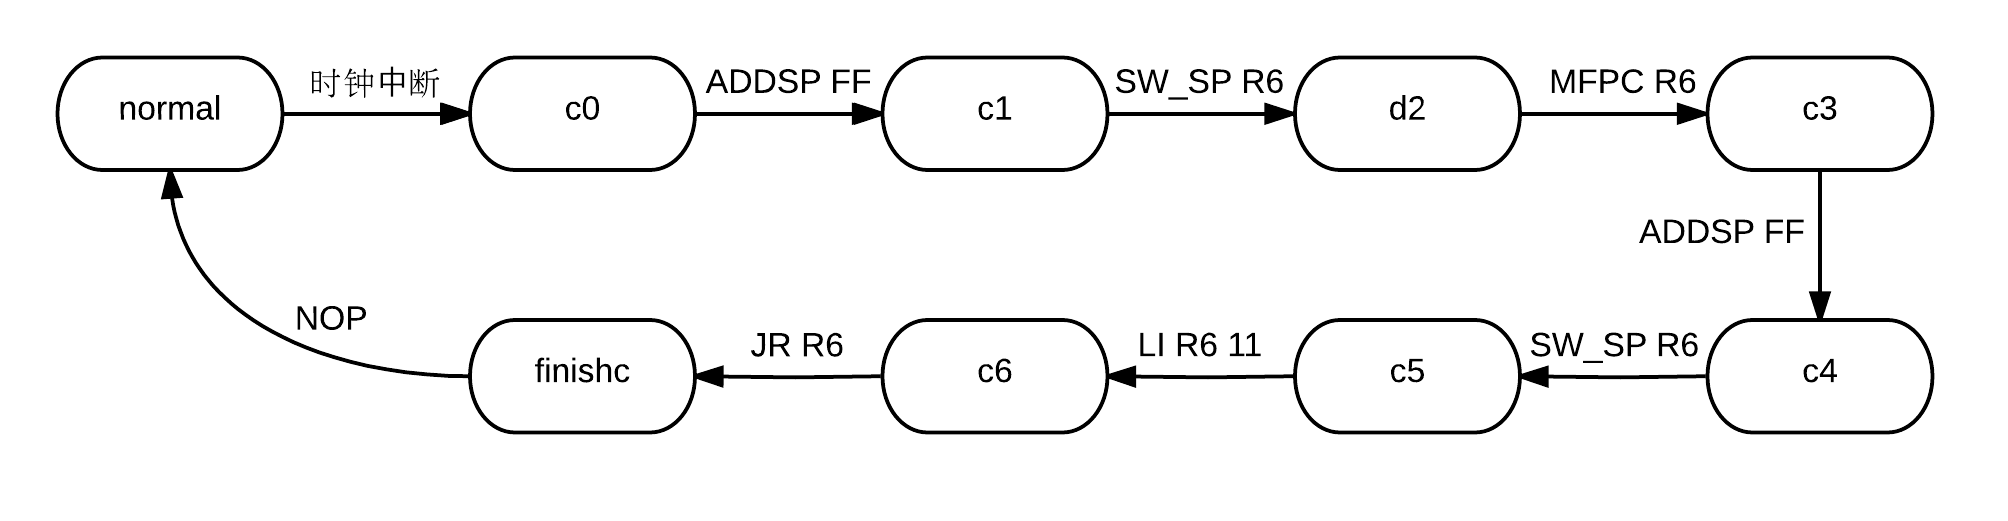
\includegraphics[width=\linewidth]{Figures/clock.png}
  \caption{时钟中断状态机.}
\end{figure}



%----------------------------------------------------------------------------------------
%	SECTION 5
%----------------------------------------------------------------------------------------

\section{I/O}

%----------------------------------------------------------------------------------------
%	SECTION 6
%----------------------------------------------------------------------------------------

\section{多道程序}


%% Chapter Template

\chapter{模块划分与接口设计} % Main chapter title

\label{Chapter4} % Change X to a consecutive number; for referencing this chapter elsewhere, use \ref{ChapterX}
本章介绍实验代码的模块划分,以及各个模块的接口设计。

%----------------------------------------------------------------------------------------
%	SECTION 1
%----------------------------------------------------------------------------------------

\section{IFetch}
读写指令模块,控制指令寄存器RAM2的读写操作,时序逻辑。同时根据输入PC和暂停流水线信号输出下一条顺序执行指令的PC值。

\begin{center}
\renewcommand{\arraystretch}{1.3}
\small
\begin{longtable}{|p{3cm}<{\centering}|p{1.4cm}<{\centering}|p{7cm}<{\centering}|}
\caption{IFetch Interface}
\label{tab:treatments}\\
\hline
接口名称 & 类型 & 功能 \\\hline
clk & in & 输入时钟 \\\hline
Ram2Addr & out & Ram2地址线\\\hline
Ram2Data & inout &  Ram2数据线\\\hline
PC & in & 输入PC \\\hline
PCInc & out & 输出PC \\\hline
IR & out & 输出指令 \\\hline
PCStop & in & 插入气泡信号\\\hline
IFWE & in & Ram2写信号\\\hline
IFData & in &  写入Ram2的数据 \\\hline
IFAddr & in & 写入Ram2的地址\\\hline
Ram2EN & out & Ram2的EN使能\\\hline
Ram2WE & out & Ram2的WE使能\\\hline
Ram2OE & out & Ram2的OE使能\\\hline
\end{longtable}
\end{center}

%----------------------------------------------------------------------------------------
%	SECTION 2
%----------------------------------------------------------------------------------------

\section{IF$\_$ID$\_$REGISTER}

IF$\_$ID段间锁存器,时序逻辑。除了传递信号外,还需处理中断,通过硬件方式保存现场并跳到中断处理程序。另外,还需要根据Forward Unit模块产生的插气泡信号和MEM产生的写RAM2信号进行停止流水线操作。

\begin{center}
\renewcommand{\arraystretch}{1.3}
\small
\begin{longtable}{|p{3cm}<{\centering}|p{1.4cm}<{\centering}|p{7cm}<{\centering}|}
\caption{IF$\_$ID$\_$REGISTER Interface}
\label{tab:treatments}\\
\hline
接口名称 & 类型 & 说明 \\
\hline
clk & in & 时钟信号 \\
\hline
INPC & in & 输入PC值 \\
\hline
INIR & inout & 输入指令值 \\
\hline
INTERRUPT & in & 中断信号,包括四种中断 \\
\hline
IFIDSTOP & in & 插入气泡信号 \\
\hline
IF$\_$FLUSH & in & 跳转指令清除延迟槽信号 \\
\hline
IF$\_$WRITE$\_$RAM2 & in & Ram2写指令,暂停流水线 \\
\hline
OUTPC & out & 输出PC值 \\
\hline
OUTIR & out &  输出指令值\\
\hline
\end{longtable}
\end{center}

%----------------------------------------------------------------------------------------
%	SECTION 3
%----------------------------------------------------------------------------------------

\section{Controller}

CPU控制器,组合逻辑。译码指令来产生控制信号。

\begin{center}
\renewcommand{\arraystretch}{1.3}
\small
\begin{longtable}{|p{3cm}<{\centering}|p{1.4cm}<{\centering}|p{7cm}<{\centering}|}
\caption{Controller Interface}
\label{tab:treatments}\\
\hline
接口名称 & 类型 & 说明 \\
\hline
INSTRUCTION & in & 需要译码的指令 \\
\hline
SRCREG1 & out & 第一个源寄存器编号 \\
\hline
SRCREG2 & out & 第二个源寄存器编号\\
\hline
TARGETREG & out & 目的寄存器编号 \\
\hline
EXTENDIMM & out & 扩展后的立即数 \\
\hline
ALUOP & out & ALU操作符 \\
\hline
ALUSRCA & out & ALU第一个操作数选择信号 \\
\hline
ALUSRCB & out & ALU第二个操作数选择信号 \\
\hline
MEMTOREG & out &  读内存信号 \\
\hline
REGWRITE & out & 写寄存器信号 \\
\hline
MEMWRITE & out & 写内存信号 \\
\hline
BRANCH & out & B型跳转信号 \\
\hline
JUMP & out & J型跳转信号 \\
\hline
\end{longtable}
\end{center}

%----------------------------------------------------------------------------------------
%	SECTION 4
%----------------------------------------------------------------------------------------

\section{RegisterCluster}

寄存器堆,存放各个寄存器的值,用于读写寄存器。写寄存器为时序逻辑,读寄存器为组合逻辑。

\begin{center}
\renewcommand{\arraystretch}{1.3}
\small
\begin{longtable}{|p{3cm}<{\centering}|p{1.4cm}<{\centering}|p{7cm}<{\centering}|}
\caption{RegisterCluster Interface}
\label{tab:treatments}\\
\hline
接口名称 & 类型 & 说明 \\
\hline
clk & in & 时钟信号 \\
\hline
rst & in & 复位信号 \\
\hline
SRCREG1 & in & 输入第一个源寄存器编号 \\
\hline
SRCREG2 & in & 输入第二个源寄存器编号 \\
\hline
TARGETREG & in & 输入目的寄存器编号 \\
\hline
REGWRITE & in & 寄存器写使能 \\
\hline
WRITEDATA & in & 写回数据 \\
\hline
REGDATA1 & out & 输出第一个源寄存器值 \\
\hline
REGDATA2 & out &  输出第二个源寄存器值\\
\hline
\end{longtable}
\end{center}

%----------------------------------------------------------------------------------------
%	SECTION 5
%----------------------------------------------------------------------------------------

\section{PC}

计算下一周期PC值的模块,组合逻辑。根据跳转信号判断和输出下一周期的跳转地址。为了兼顾B指令、J指令的各种情况,输入多个可能的跳转地址,包括旁路信号。

\begin{center}
\renewcommand{\arraystretch}{1.3}
\small
\begin{longtable}{|p{3cm}<{\centering}|p{1.4cm}<{\centering}|p{7cm}<{\centering}|}
\caption{PC Interface}
\label{tab:treatments}\\
\hline
接口名称 & 类型 & 说明 \\
\hline
CURRENTPC & in & 当前PC \\
\hline
LASTPC & in & 上一周期的PC \\
\hline
EXTENDIMM & in & B指令的偏移值 \\
\hline
BRANCH & in & B指令跳转类型 \\
\hline
JUMP & in & J指令跳转 \\
\hline
REG1data & in & 寄存器值,对B指令可用于判断是否跳转,对J指令指定跳转地址 \\
\hline
ALURES1 & in & ALU阶段旁路值 \\
\hline
ALURES2 & in & MEM阶段保存的ALU结果 \\
\hline
MEMDATA & in &  MEM阶段读取的内存值 \\
\hline
FORWARD & in & 数据冲突信号 \\
\hline
NEXTPC & out & 下一指令PC值 \\
\hline
IF$\_$FLUSH & out & 清除延迟槽信号 \\
\hline
\end{longtable}
\end{center}
%\end{table}

%----------------------------------------------------------------------------------------
%	SECTION 6
%----------------------------------------------------------------------------------------

\section{ID$\_$EX$\_$REGISTER}

ID$\_$EXE段间锁存器,时序逻辑。传递信号,还需根据FORWARD UNIT模块的插气泡信号暂停流水线。

\begin{center}
\renewcommand{\arraystretch}{1.3}
\small
\begin{longtable}{|p{3cm}<{\centering}|p{1.4cm}<{\centering}|p{7cm}<{\centering}|}
\caption{ID$\_$EX$\_$REGISTER Interface}
\label{tab:treatments}\\
\hline
接口名称 & 类型 & 说明 \\
\hline
clk & in & 时钟信号 \\
\hline
CONTROLSTOP & in & 暂停流水线信号 \\
\hline
IN$\_$MEMTOREG & in & 输入读内存信号 \\
\hline
IN$\_$REGWRITE & in & 输入写寄存器信号 \\
\hline
IN$\_$MEMWRITE & in & 输入写内存信号 \\
\hline
IN$\_$ALUSRCA & in & 输入ALU第一个操作数选择信号 \\
\hline
IN$\_$ALUSRCB & in & 输入ALU第二个操作数选择信号 \\
\hline
IN$\_$ALUOP & in & 输入ALU操作符 \\
\hline
IN$\_$FORWARDA & in & 输入数据旁路选择信号A \\
\hline
IN$\_$FORWARDB & in & 输入数据旁路选择信号B \\
\hline
IN$\_$EXTENDIMM & in & 输入扩展的立即数 \\
\hline
IN$\_$TARGETREG & in & 输入写回寄存器编号 \\
\hline
IN$\_$REGDATA1 & in & 输入第一个寄存器值 \\
\hline
IN$\_$REGDATA2 & in & 输入第二个寄存器值 \\
\hline
IN$\_$PC & in & 输入PC值 \\
\hline
OUT$\_$MEMTOREG & out & 输出读内存信号 \\
\hline
OUT$\_$REGWRITE & out & 输出写寄存器信号 \\
\hline
OUT$\_$MEMWRITE & out & 输出写内存信号 \\
\hline
OUT$\_$ALUSRCA & out & 输出ALU第一个操作数选择信号 \\
\hline
OUT$\_$ALUSRCB & out & 输出ALU第二个操作数选择信号 \\
\hline
OUT$\_$ALUOP & out & 输出ALU运算符  \\
\hline
OUT$\_$FORWARDA & out & 输出数据旁路选择信号A \\
\hline
OUT$\_$FORWARDB & out & 输出数据旁路选择信号B \\
\hline
OUT$\_$EXTENDIMM & out & 输出扩展的立即数 \\
\hline
OUT$\_$TARGETREG & out & 输出写回寄存器编号 \\
\hline
OUT$\_$REGDATA1 & out & 输出第一个寄存器值 \\
\hline
OUT$\_$REGDATA2 & out & 输出第二个寄存器值 \\
\hline
OUT$\_$PC & out & 输出PC值 \\
\hline
\end{longtable}
\end{center}

%----------------------------------------------------------------------------------------
%	SECTION 7
%----------------------------------------------------------------------------------------

\section{ALU}

ALU运算器,组合逻辑。用于EXE阶段进行运算。

\begin{center}
\renewcommand{\arraystretch}{1.3}
\small
\begin{longtable}{|p{3cm}<{\centering}|p{1.4cm}<{\centering}|p{7cm}<{\centering}|}
\caption{ALU Interface}
\label{tab:treatments}\\
\hline
接口名称 & 类型 & 说明 \\
\hline
REGDATA1 & in & 第一个寄存器的值 \\
\hline
REGDATA2 & in & 第二个寄存器的值 \\
\hline
EXTENDIMM & in & 扩展的立即数 \\
\hline
LASTALU & in & 上一条指令ALU结果 \\
\hline
LASTMEM & in & 上两条指令MEM结果 \\
\hline
forwardA & in & 第一个运算数的数据冲突选择信号 \\
\hline
forwardB & in & 第二个运算数的数据冲突选择信号 \\
\hline
ALUSRCA & in & 第一个运算数的选择信号 \\
\hline
ALUSRCB & in &  第二个运算数的选择信号 \\
\hline
ALUOP & in & ALU运算符 \\
\hline
PC & in & PC值 \\
\hline
ALURES & out & ALU结果 \\
\hline
REGDATA & out & 选择的寄存器值,用于写到内存 \\
\hline
\end{longtable}
\end{center}

%----------------------------------------------------------------------------------------
%	SECTION 8
%----------------------------------------------------------------------------------------

\section{EX$\_$MEM$\_$REGISTER}

EXE$\_$MEM段间锁存器,时序逻辑。

\begin{center}
\renewcommand{\arraystretch}{1.3}
\small
\begin{longtable}{|p{3cm}<{\centering}|p{1.4cm}<{\centering}|p{7cm}<{\centering}|}
\caption{EX$\_$MEM$\_$REGISTER Interface}
\label{tab:treatments}\\
\hline
接口名称 & 类型 & 说明 \\
\hline
clk & in & 时钟信号 \\
\hline
IN$\_$MEMTOREG & in & 输入读内存信号 \\
\hline
IN$\_$REGWRITE & in & 输入写寄存器信号 \\
\hline
IN$\_$MEMWRITE & in & 输入写内存信号 \\
\hline
IN$\_$ALURES & in & 输入ALU计算结果 \\
\hline
IN$\_$REGDATA & in & 输入MEM写入数据 \\
\hline
IN$\_$TARGETREG & in & 输入目的寄存器编号 \\
\hline
OUT$\_$MEMTOREG & out & 输出读内存信号 \\
\hline
OUT$\_$REGWRITE & out & 输出写寄存器信号 \\
\hline
OUT$\_$MEMWRITE & out & 输出写内存信号 \\
\hline
OUT$\_$ALURES & out & 输出ALU计算结果 \\
\hline
OUT$\_$REGDATA & out & 输出MEM写入数据 \\
\hline
OUT$\_$TARGETREG & out & 输出目的寄存器编号 \\
\hline
\end{longtable}
\end{center}

%----------------------------------------------------------------------------------------
%	SECTION 9
%----------------------------------------------------------------------------------------

\section{MEM}

访存阶段模块,控制数据寄存器Ram1的读写,时序逻辑。此模块中还需根据读写地址判断是否为写入指令、读写串口、键盘vga读写等等。

\begin{center}
\renewcommand{\arraystretch}{1.3}
\small
\begin{longtable}{|p{3cm}<{\centering}|p{1.4cm}<{\centering}|p{7cm}<{\centering}|}
\caption{MEM Interface}
\label{tab:treatments}\\
\hline
接口名称 & 类型 & 说明 \\
\hline
clk & in & 输入时钟\\
\hline
Ram1Data & inout & Ram1数据线 \\
\hline
Ram1Addr & out & Ram1地址线 \\
\hline
Ram1OE & out & Ram1的OE使能\\
\hline
Ram1WE & out & Ram1的WE使能 \\
\hline
Ram1EN & out & Ram1的EN使能 \\
\hline
data$\_$ready & in & 键盘的data\_ready信号 \\
\hline
tbre & in & VGA模块的tbre信号 \\
\hline
tsre & in & VGA模块的tsre信号 \\
\hline
rdn & out &  给键盘的rdn控制信号 \\
\hline
wrn & out & 给VGA模块的wrn控制信号 \\
\hline
uart$\_$data$\_$ready & in & 串口的data\_ready信号 \\
\hline
uart$\_$tbre & in & 串口的tbre信号 \\
\hline
uart$\_$tsre & in & 串口的tsre信号 \\
\hline
uart$\_$rdn & out & 串口的rdn控制信号 \\
\hline
uart$\_$wrn & out & 串口的wrn控制信号 \\
\hline
MemData & in & 输入的数据线\\
\hline
MemAddr & in & 输入的地址线\\
\hline
MemWE & in & 写信号\\
\hline
MemRE & in & 读信号\\
\hline
IFWE & out & 控制是否写Ram2的信号\\
\hline 
IFData & out & 给Ram2的数据\\
\hline
IFAddr & out & 给Ram2的地址\\
\hline
\end{longtable}
\end{center}


%----------------------------------------------------------------------------------------
%	SECTION 10
%----------------------------------------------------------------------------------------

\section{MEM$\_$WB$\_$REGISTER}

MEM$\_$WE段间锁存器,时序逻辑。

\begin{center}
\renewcommand{\arraystretch}{1.3}
\small
\begin{longtable}{|p{3cm}<{\centering}|p{1.4cm}<{\centering}|p{7cm}<{\centering}|}
\caption{MEM$\_$WB$\_$REGISTER Interface}
\label{tab:treatments}\\
\hline
接口名称 & 类型 & 说明 \\
\hline
clk & in & 时钟信号 \\
\hline
IN$\_$MEMTOREG & in & 输入内存数据写入寄存器信号 \\
\hline
IN$\_$REGWRITE & in & 输入写寄存器信号 \\
\hline
ALURES & in & 输入ALU计算结果 \\
\hline
IN$\_$TARGETREG & in & 输入目的寄存器编号 \\
\hline
READDATA & in & 内存读出的数据 \\
\hline
OUT$\_$REGWRITE & out & 输出写寄存器信号 \\
\hline
OUT$\_$TARGETREG & out & 输出目的寄存器编号 \\
\hline
WRITEDATA & out & 写回数据 \\
\hline
\end{longtable}
\end{center}

%----------------------------------------------------------------------------------------
%	SECTION 11
%----------------------------------------------------------------------------------------

\section{FORFARD\_UNIT}

数据冲突检测模块,组合逻辑。根据当前ID阶段指令的源寄存器编号与EXE、MEM阶段的目的寄存器编号是否相等及写回寄存器、读写内存等信号判断是否发生数据冲突及是否需要插气泡。

\begin{center}
\renewcommand{\arraystretch}{1.3}
\small
\begin{longtable}{|p{3cm}<{\centering}|p{1.4cm}<{\centering}|p{7cm}<{\centering}|}
\caption{FORFARD\_UNIT Interface}
\label{tab:treatments}\\
\hline
接口名称 & 类型 & 说明 \\
\hline
SRCREG1 & in & ID阶段源寄存器1编号 \\
\hline
SRCREG2 & in & ID阶段源寄存器2编号 \\
\hline
TARGETREGALU & in & ALU阶段目的寄存器编号 \\
\hline
TARGETREGMEM & in & MEM阶段目的寄存器编号 \\
\hline
REGWRITEALU & in & ALU阶段写回寄存器信号 \\
\hline
MEMTOREGALU & in & ALU阶段读内存信号 \\
\hline
REGWRITEMEM & in & MEM阶段写回寄存器信号 \\
\hline
MEMTOREGMEM & in & MEM阶段读内存信号 \\
\hline
FORWARDA & out & 当前指令ALU操作数1数据冲突选择信号 \\
\hline
FORWARDB & out & 当前指令ALU操作数2数据冲突选择信号\\
\hline
FORWARD & out & 当前指令跳转时数据冲突选择信号\\
\hline
PCSTOP & out & 插入气泡\\
\hline
IFIDSTOP & out & 插入气泡\\
\hline
CONTROLSTOP & out & 插入气泡\\
\hline
\end{longtable}
\end{center}

%----------------------------------------------------------------------------------------
%	SECTION 12
%----------------------------------------------------------------------------------------

\section{Keyboard}

用于键盘读入,通过状态机来接收通码、断码,并做奇偶校验。将得到的键盘输入输出到keyboardCpuRam模块进行处理。

\begin{center}
\renewcommand{\arraystretch}{1.3}
\small
\begin{longtable}{|p{3cm}<{\centering}|p{1.4cm}<{\centering}|p{7cm}<{\centering}|}
\caption{Keyboard Interface}
\label{tab:treatments}\\
\hline
接口名称 & 类型 & 说明 \\
\hline
datain & in & 键盘输入数据 \\
\hline
clkin & in & 键盘时钟 \\
\hline
fclk & in & 50M时钟 \\
\hline
interrupt & out & ESC中断信号 \\
\hline
interruptC & out & Control C中断信号 \\
\hline
keyboard$\_$out & out & 键盘输入结束信号 \\
\hline
shiftstate & out & shift组合键 \\
\hline
ctrlstate & out & ctrl组合键\\
\hline
word & out & 键盘数据\\
\hline
\end{longtable}
\end{center}

%----------------------------------------------------------------------------------------
%	SECTION 13
%----------------------------------------------------------------------------------------

\section{KeyboardCpuRam}

模拟term程序的输入部分,通过键盘的摁键设置状态机,实现A、G、U、D、R五条term程序指令,并发送给CPU模块。

\begin{center}
\renewcommand{\arraystretch}{1.3}
\small
\begin{longtable}{|p{3cm}<{\centering}|p{1.4cm}<{\centering}|p{7cm}<{\centering}|}
\caption{KeyboardCpuRam Interface}
\label{tab:treatments}\\
\hline
接口名称 & 类型 & 说明 \\
\hline
clk50 & in & 50M时钟 \\
\hline
KeyBoardData & in & 键盘输入到状态机的数据 \\
\hline
DataReady & in & 键盘输入至状态机的通知 \\
\hline
CpuDataReady & out & 状态机输入到主机 \\
\hline
DataPath & inout & 数据总线 \\
\hline
CpuRdn & in & 主机给状态机读信号 \\
\hline
CpuEnable & in & 主机给状态机是否能写\\
\hline
RamData & out & 将acsii字符写入ram,用于VGA显示\\
\hline
RamDataReady & out & dataready给ram \\
\hline
RamRdn & in & ram给状态机的通知 \\
\hline
 shiftstat & in & shift组合键信号 \\
 \hline
 ctrlstate & in & ctrl组合键信号 \\
 \hline
\end{longtable}
\end{center}

%----------------------------------------------------------------------------------------
%	SECTION 14
%----------------------------------------------------------------------------------------

\section{KeyboardStateMachine}

键盘输入部分的top模块。用于与CPU和VGA进行通信,同时访问底层keyboard模块数据,保证数据的正确性。

\begin{center}
\renewcommand{\arraystretch}{1.3}
\small
\begin{longtable}{|p{3cm}<{\centering}|p{1.4cm}<{\centering}|p{7cm}<{\centering}|}
\caption{KeyboardStateMachine Interface}
\label{tab:treatments}\\
\hline
接口名称 & 类型 & 说明 \\
\hline
datain & in & 键盘输入数据 \\
\hline
clkin & in & 键盘时钟 \\
\hline
fclk & in & 50M时钟 \\
\hline
interrupt & out & ESC中断信号 \\
\hline
interruptC & out & Control C中断信号 \\
\hline
rdn & in & 主机给状态机的读信号 \\
\hline
CpuDataReady & out & 键盘给主机可读信号 \\
\hline
showData & inout & 键盘给CPU的数据 \\
\hline
KBData & out & 键盘给VGA的数据\\
\hline
KBdata$\_$ready & out & 键盘给VGA可读信号\\
\hline
KBrdn & in & VGA给键盘读使能 \\
\hline
\end{longtable}
\end{center}

%----------------------------------------------------------------------------------------
%	SECTION 15
%----------------------------------------------------------------------------------------

\section{Compiler}

汇编代码转为机器码的模块。当term执行A指令时,用户可以输入汇编码,键盘模块将整句的汇编码保存在缓冲区中,等待回车到来后将输入的汇编码转为机器码,并发送到CPU以写入RAM2.

\begin{center}
\renewcommand{\arraystretch}{1.3}
\small
\begin{longtable}{|p{3cm}<{\centering}|p{1.4cm}<{\centering}|p{7cm}<{\centering}|}
\caption{Compiler Interface}
\label{tab:treatments}\\
\hline
接口名称 & 类型 & 说明 \\
\hline
sendbuffer & in & 输入指令缓冲区 \\
\hline
instruc & out & 16位指令机器码表示 \\
\hline
\end{longtable}
\end{center}

%----------------------------------------------------------------------------------------
%	SECTION 16
%----------------------------------------------------------------------------------------

\section{VGA\_Controller}

VGA控制模块,控制计算机的VGA显示功能,主要任务是将需要显示的数据存入显存(一块FPGA片内RAM),并控制VGA的显示。

\begin{center}
\renewcommand{\arraystretch}{1.3}
\small
\begin{longtable}{|p{3cm}<{\centering}|p{1.4cm}<{\centering}|p{7cm}<{\centering}|}
\caption{VGA\_Controller Interface}
\label{tab:treatments}\\
\hline
接口名称 & 类型 & 说明 \\\hline
clk50 & in & 50M时钟 \\\hline
rst & in  & 复位信号 \\\hline
DataIn & in  & 输入数据 \\\hline
data\_ready & in & VGA的data\_ready信号\\\hline
rdn & out  & VGA的rdn控制信号 \\\hline
hs & out & VGA行同步信号\\\hline
vs & out & VGA场同步信号\\\hline
r, g, b & out & VGA输出的RGB \\\hline
\end{longtable}
\end{center}

%----------------------------------------------------------------------------------------
%	SECTION 17
%----------------------------------------------------------------------------------------

\section{VGA}

VGA模块,控制VGA输出,包括从一块FPGA片内ROM中读取字符图片并显示。

\begin{center}
\renewcommand{\arraystretch}{1.3}
\small
\begin{longtable}{|p{3cm}<{\centering}|p{1.4cm}<{\centering}|p{7cm}<{\centering}|}
\caption{VGA\_Controller Interface}
\label{tab:treatments}\\
\hline
接口名称 & 类型 & 说明 \\\hline
clk50 & in & 50M时钟 \\\hline
rst & in  & 复位信号 \\\hline
DataIn & in  & 输入数据 \\\hline
data\_ready & in & VGA的data\_ready信号\\\hline
hs & out & VGA行同步信号\\\hline
vs & out & VGA场同步信号\\\hline
r, g, b & out & VGA输出的RGB \\\hline
row & out & 字符行 \\\hline
column & out & 字符列 \\\hline
data & in & 一个像素的色彩值 \\\hline
\end{longtable}
\end{center}

%----------------------------------------------------------------------------------------
%	SECTION 18
%----------------------------------------------------------------------------------------

\section{VGA\_Core\_Ball}

屏幕保护显示模块,控制在屏幕保护阶段的VGA输出。这一部分代码由作者上一学期《数字逻辑设计》课程的课程项目经过精简后得到。

\begin{center}
\renewcommand{\arraystretch}{1.3}
\small
\begin{longtable}{|p{3cm}<{\centering}|p{1.4cm}<{\centering}|p{7cm}<{\centering}|}
\caption{VGA\_Core\_Ball Interface}
\label{tab:treatments}\\
\hline
接口名称 & 类型 & 说明 \\\hline
clk & in & 25M时钟输入 \\\hline
reset & in  & 复位信号 \\\hline
r, g, b & out & 输出的RGB \\\hline
vector\_x & in & 当前VGA输出的行 \\\hline
vector\_y & in & 当前VGA输出的列 \\\hline
num\_c & in & 小球个数 \\\hline
theta\_c & in & 小球角度 \\\hline
mtime  & in & 时间 \\\hline
\end{longtable}
\end{center}


%----------------------------------------------------------------------------------------
%	SECTION 19
%----------------------------------------------------------------------------------------

\section{Output\_Adaptor}

输出转换接口模块。VGA的显示有来自CPU和来自键盘两个不同的来源,经过这个模块的处理整合后提供给VGA控制模块。

\begin{center}
\renewcommand{\arraystretch}{1.3}
\small
\begin{longtable}{|p{3cm}<{\centering}|p{1.4cm}<{\centering}|p{7cm}<{\centering}|}
\caption{Output\_Adaptor Interface}
\label{tab:treatments}\\
\hline
接口名称 & 类型 & 说明 \\\hline
clk50 & in & 50M时钟 \\\hline
CPUData & in & CPU的数据 \\\hline
CPUwrn & in  & CPU的wrn信号 \\\hline
CPUtsre & out  & CPU的tsre信号 \\\hline
KBData & in  & 键盘的数据 \\\hline
KBdata\_ready & in & 键盘的data\_ready \\\hline
KBrdn & out & 键盘的rdn信号 \\\hline
DataOut & out & 输出的数据 \\\hline
data\_ready & out & 输出的data\_ready信号 \\\hline
rdn & in & rdn控制信号 \\\hline
\end{longtable}
\end{center}

 
%% Chapter Template

\chapter{实验成果} % Main chapter title

\label{Chapter5} % Change X to a consecutive number; for referencing this chapter elsewhere, use \ref{ChapterX}
我们最终的成果分为三个版本,其中包括基础功能的CPU,与键盘VGA交互的CPU,同时运行两套监控程序的CPU。下面将列举实验的一些成果。

%----------------------------------------------------------------------------------------
%	SECTION 1
%----------------------------------------------------------------------------------------

\section{基础版本CPU}

我们CPU使用的时钟为25M,可以正确执行30条指令,并对冲突有很好地处理。根据测试样例程序的的指令总数和运行时间,可以看出我们的CPU主频确实达到了25M。

\begin{figure}[H]
  \centering
  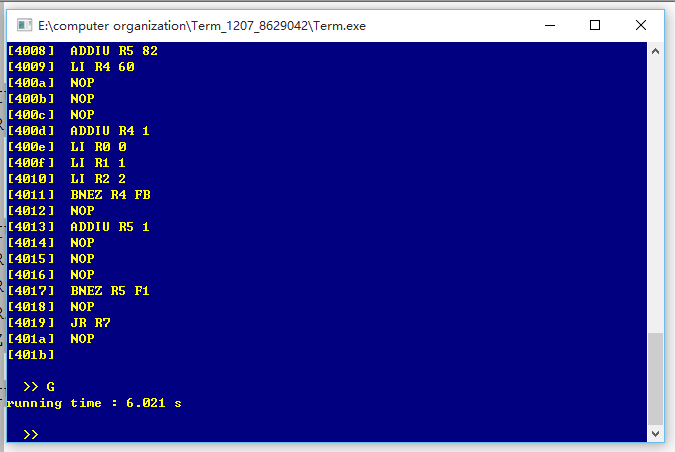
\includegraphics[width=5in]{Figures/cpu1.png}
  \caption{测试程序1}
\end{figure}

\begin{figure}[H]
  \centering
  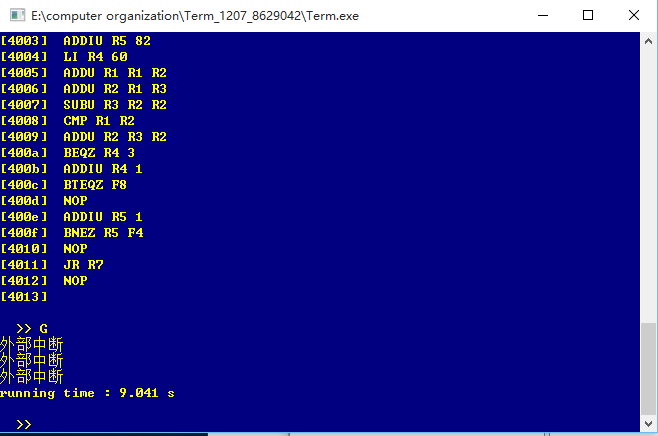
\includegraphics[width=5in]{Figures/cpu2.png}
  \caption{测试程序2}
\end{figure}

\begin{figure}[H]
  \centering
  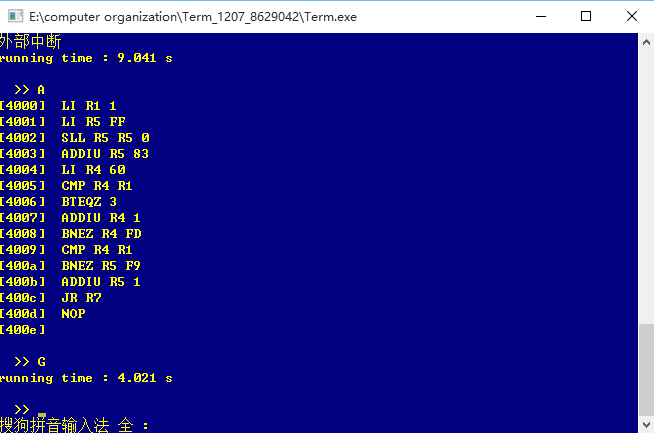
\includegraphics[width=5in]{Figures/cpu3.png}
  \caption{测试程序3}
\end{figure}

\begin{figure}[H]
  \centering
  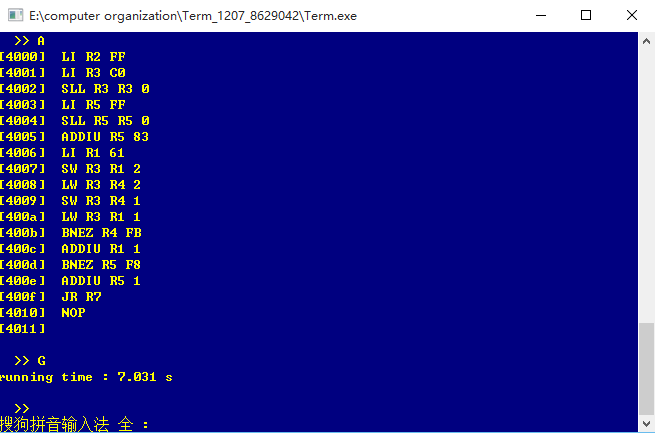
\includegraphics[width=5in]{Figures/cpu4.png}
  \caption{测试程序4}
\end{figure}

\begin{figure}[H]
  \centering
  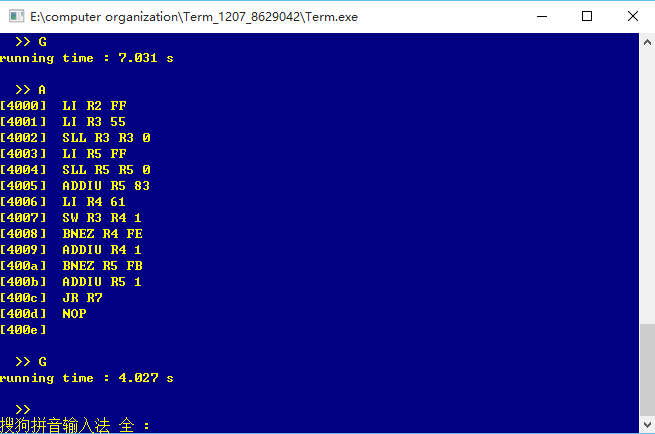
\includegraphics[width=5in]{Figures/cpu5.png}
  \caption{测试程序5}
\end{figure}

在测试程序2中,我们在运行期间通过手动clk产生中断信号,可以看到term中出现了“硬件中断”字样。

%----------------------------------------------------------------------------------------
%	SECTION 2
%----------------------------------------------------------------------------------------

\section{键盘VGA版本CPU}

键盘VGA版本的CPU并没有改变CPU内核代码,所以时钟仍为25M。以下为我们拍摄的一些实验结果。

运行程序,可以看到VGA上显示出OK字样。并通过R指令查用户寄存器的值。后面我们通过键盘输入组合键,可以看到VGA可以正确地显示出字符。

\begin{figure}[H]
  \centering
  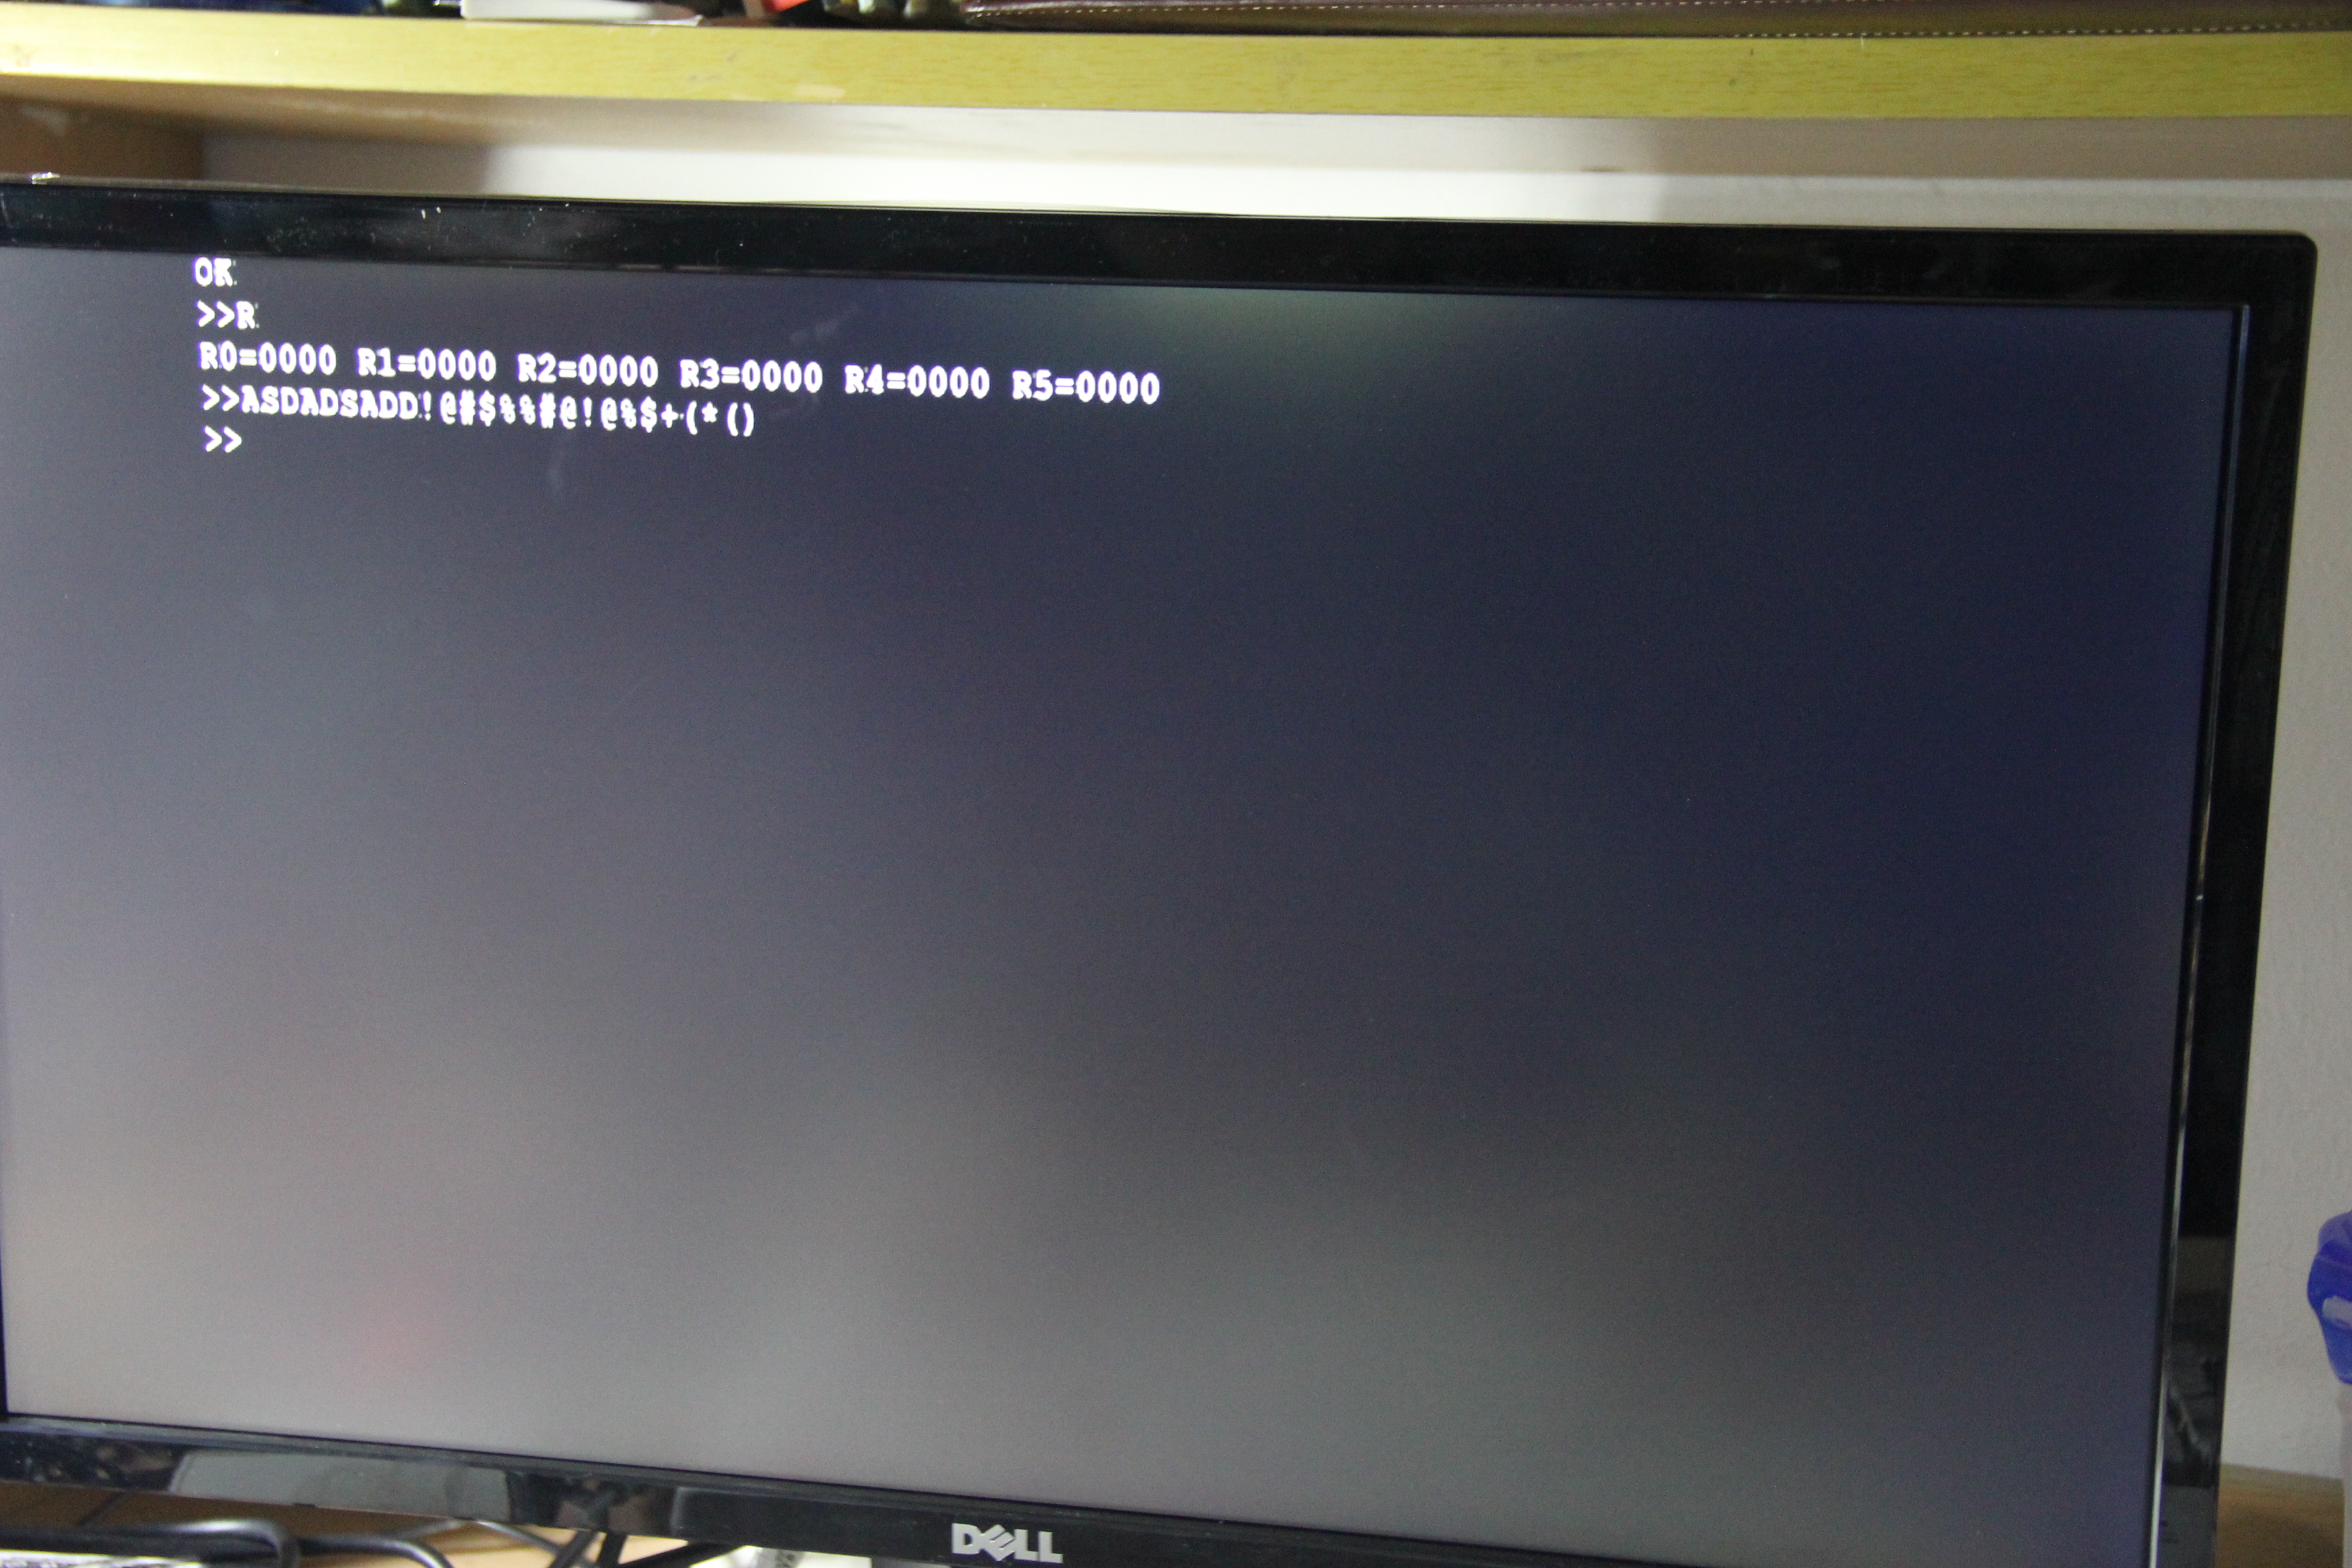
\includegraphics[width=4.5in]{Figures/picture/IMG_7232.JPG}
  \caption{R指令}
\end{figure}

我们在几秒钟没有操作之后,进入屏幕保护界面。

\begin{figure}[H]
  \centering
  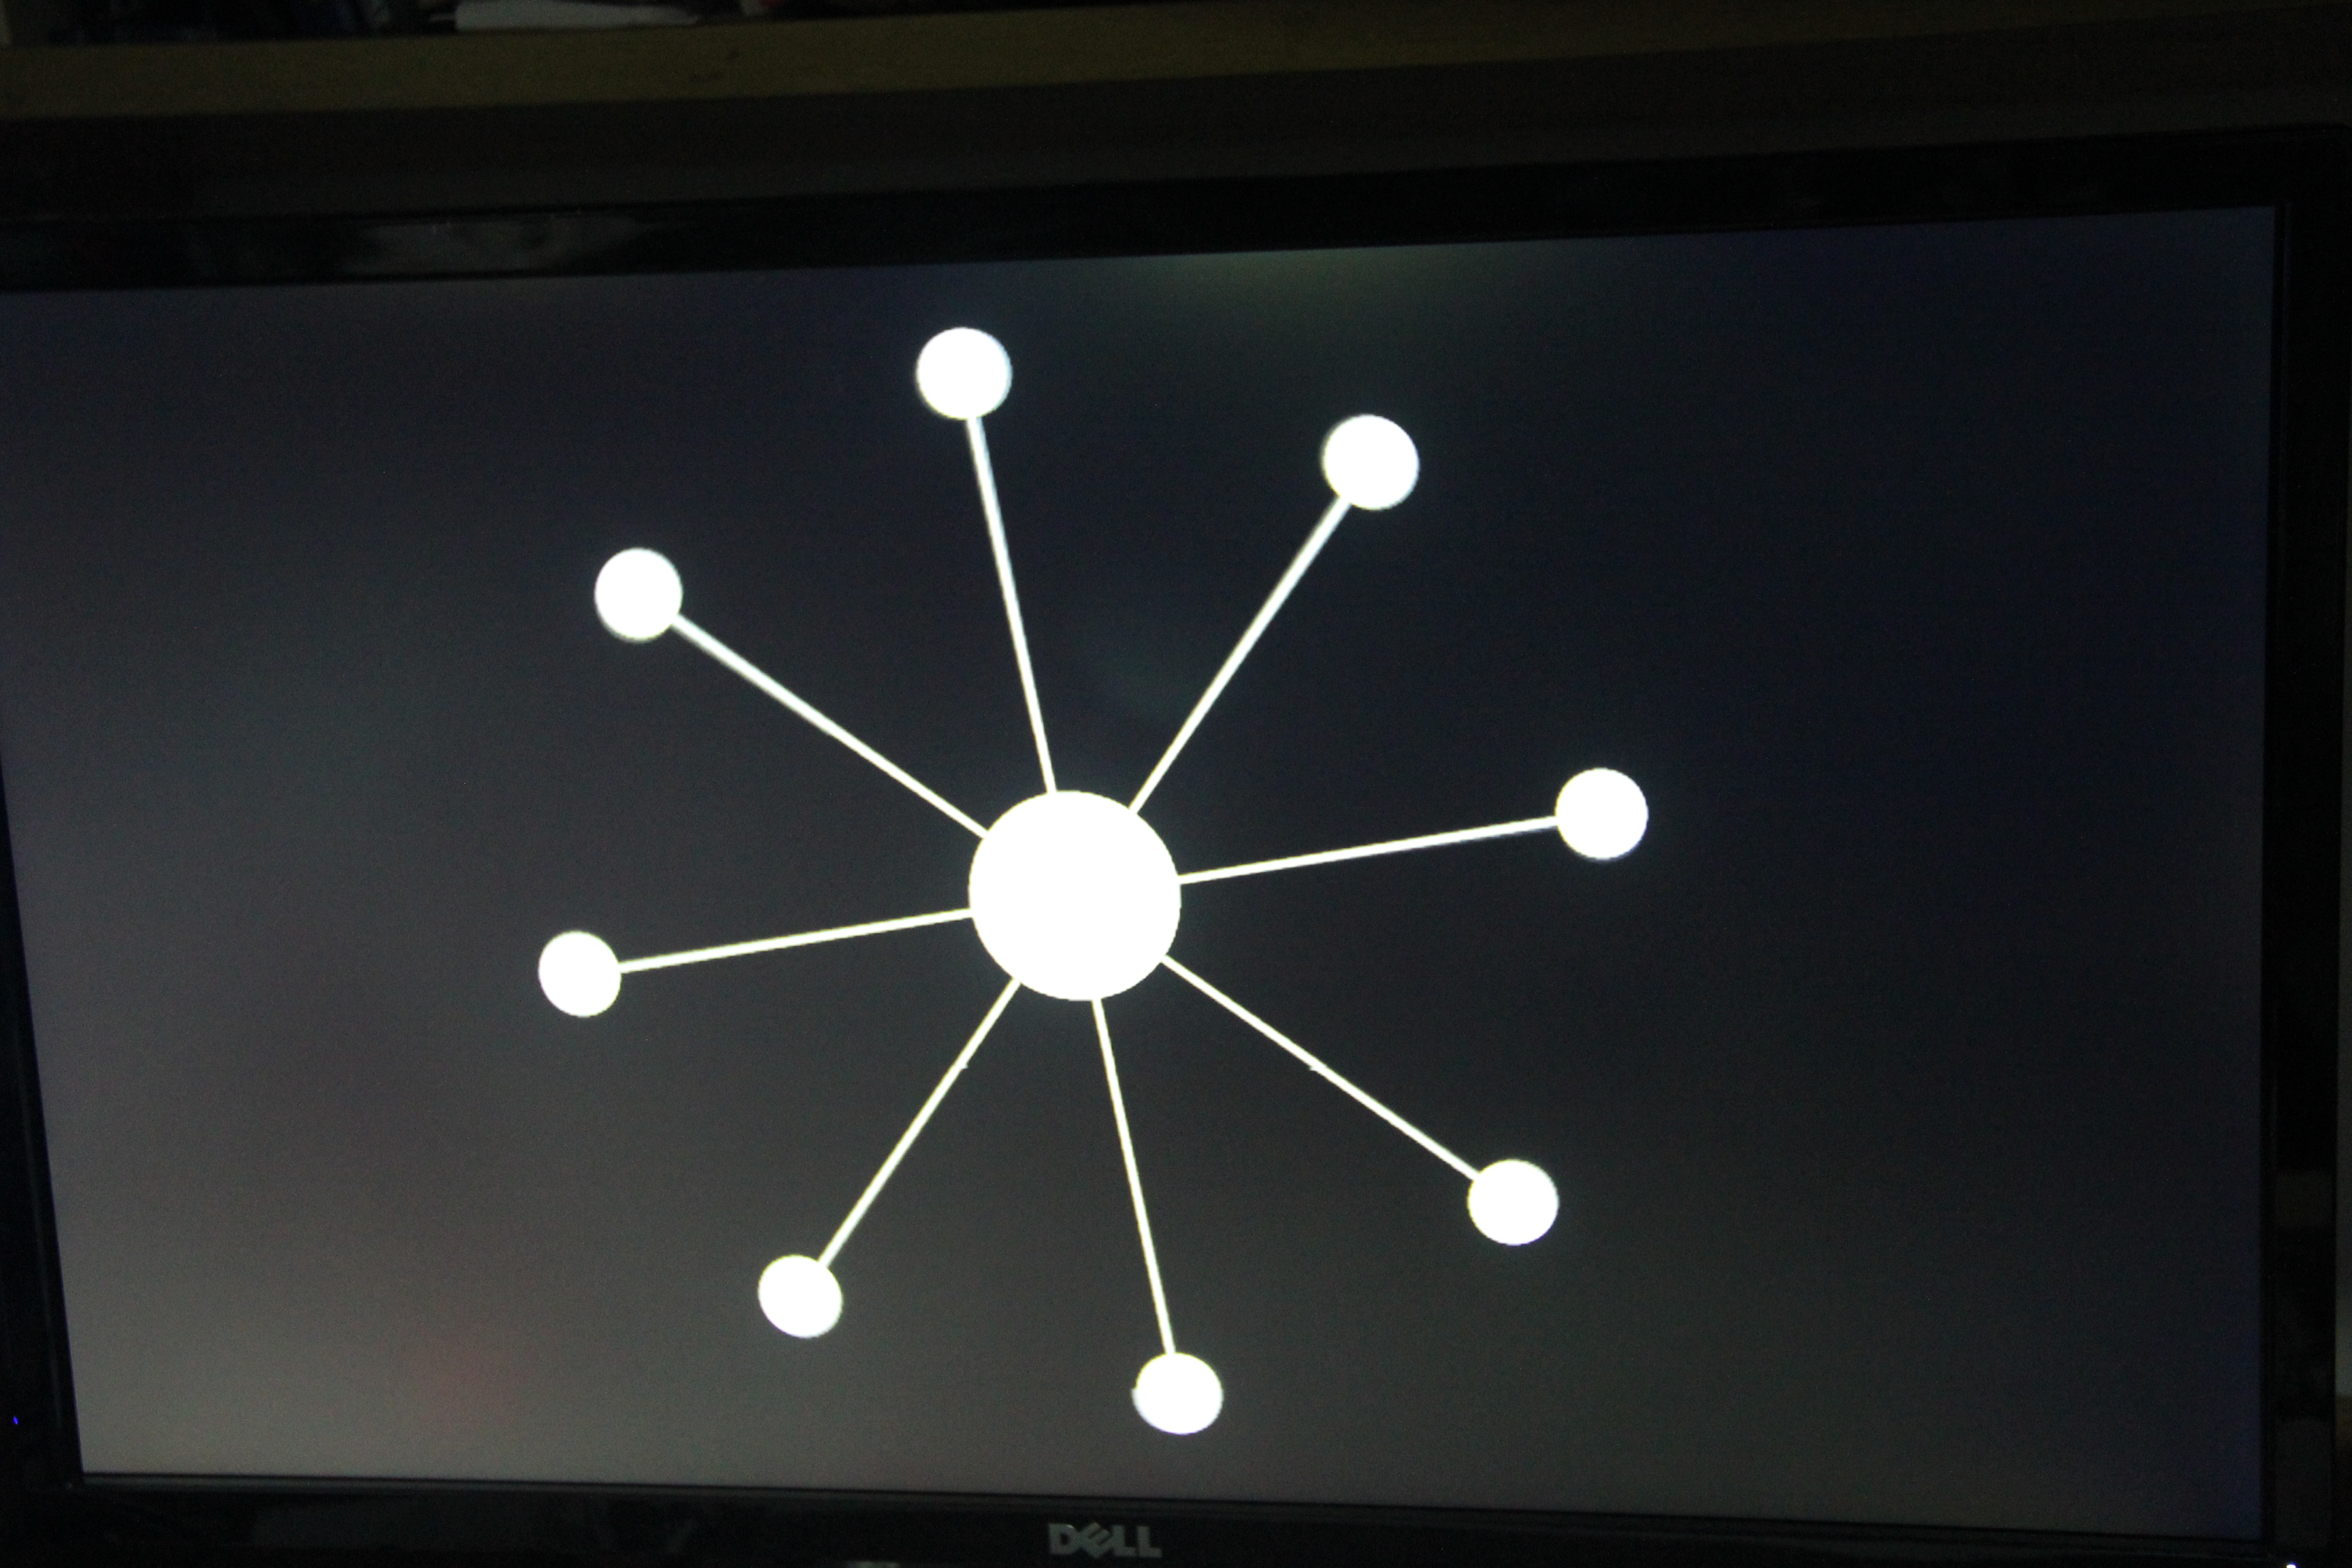
\includegraphics[width=4.5in]{Figures/picture/IMG_7233.JPG}
  \caption{屏幕保护}
\end{figure}

我们通过A指令写入汇编代码,A指令同时支持增加写入地址的参数。同时,我们通过U指令反汇编出刚写入的指令,检查正确性。

\begin{figure}[H]
  \centering
  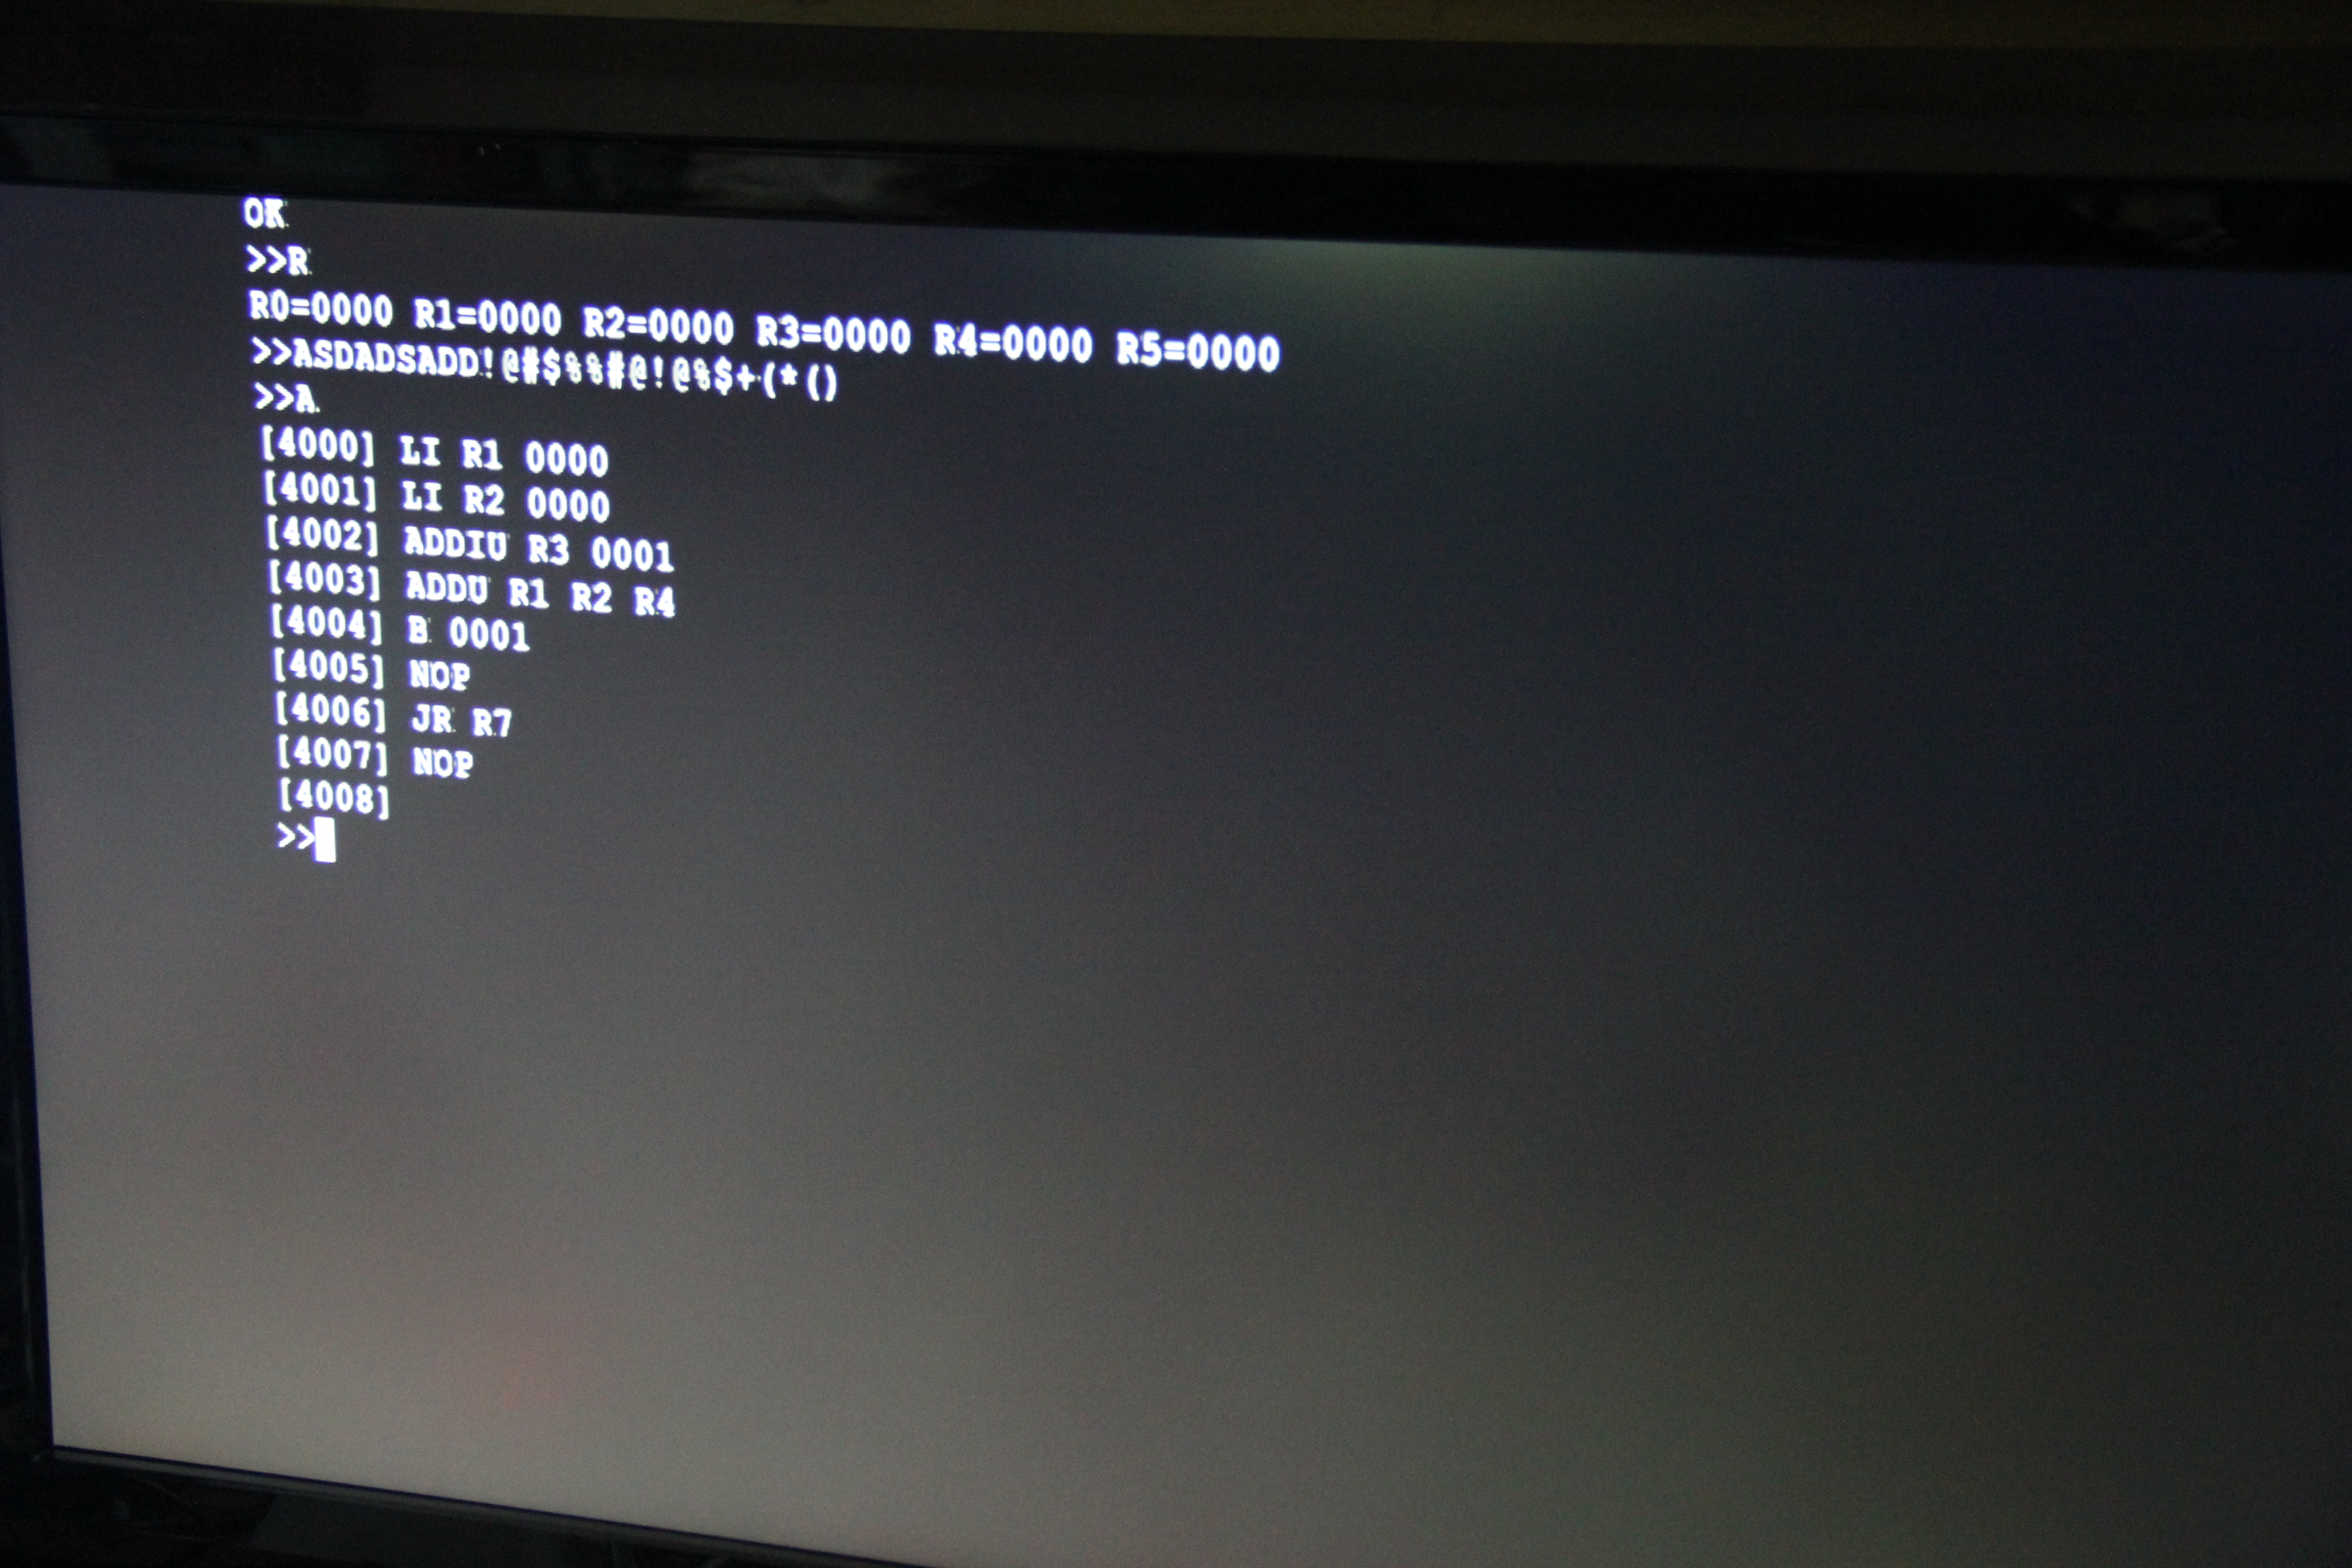
\includegraphics[width=4.5in]{Figures/picture/IMG_7235.JPG}
  \caption{A指令}
\end{figure}

\begin{figure}[H]
  \centering
  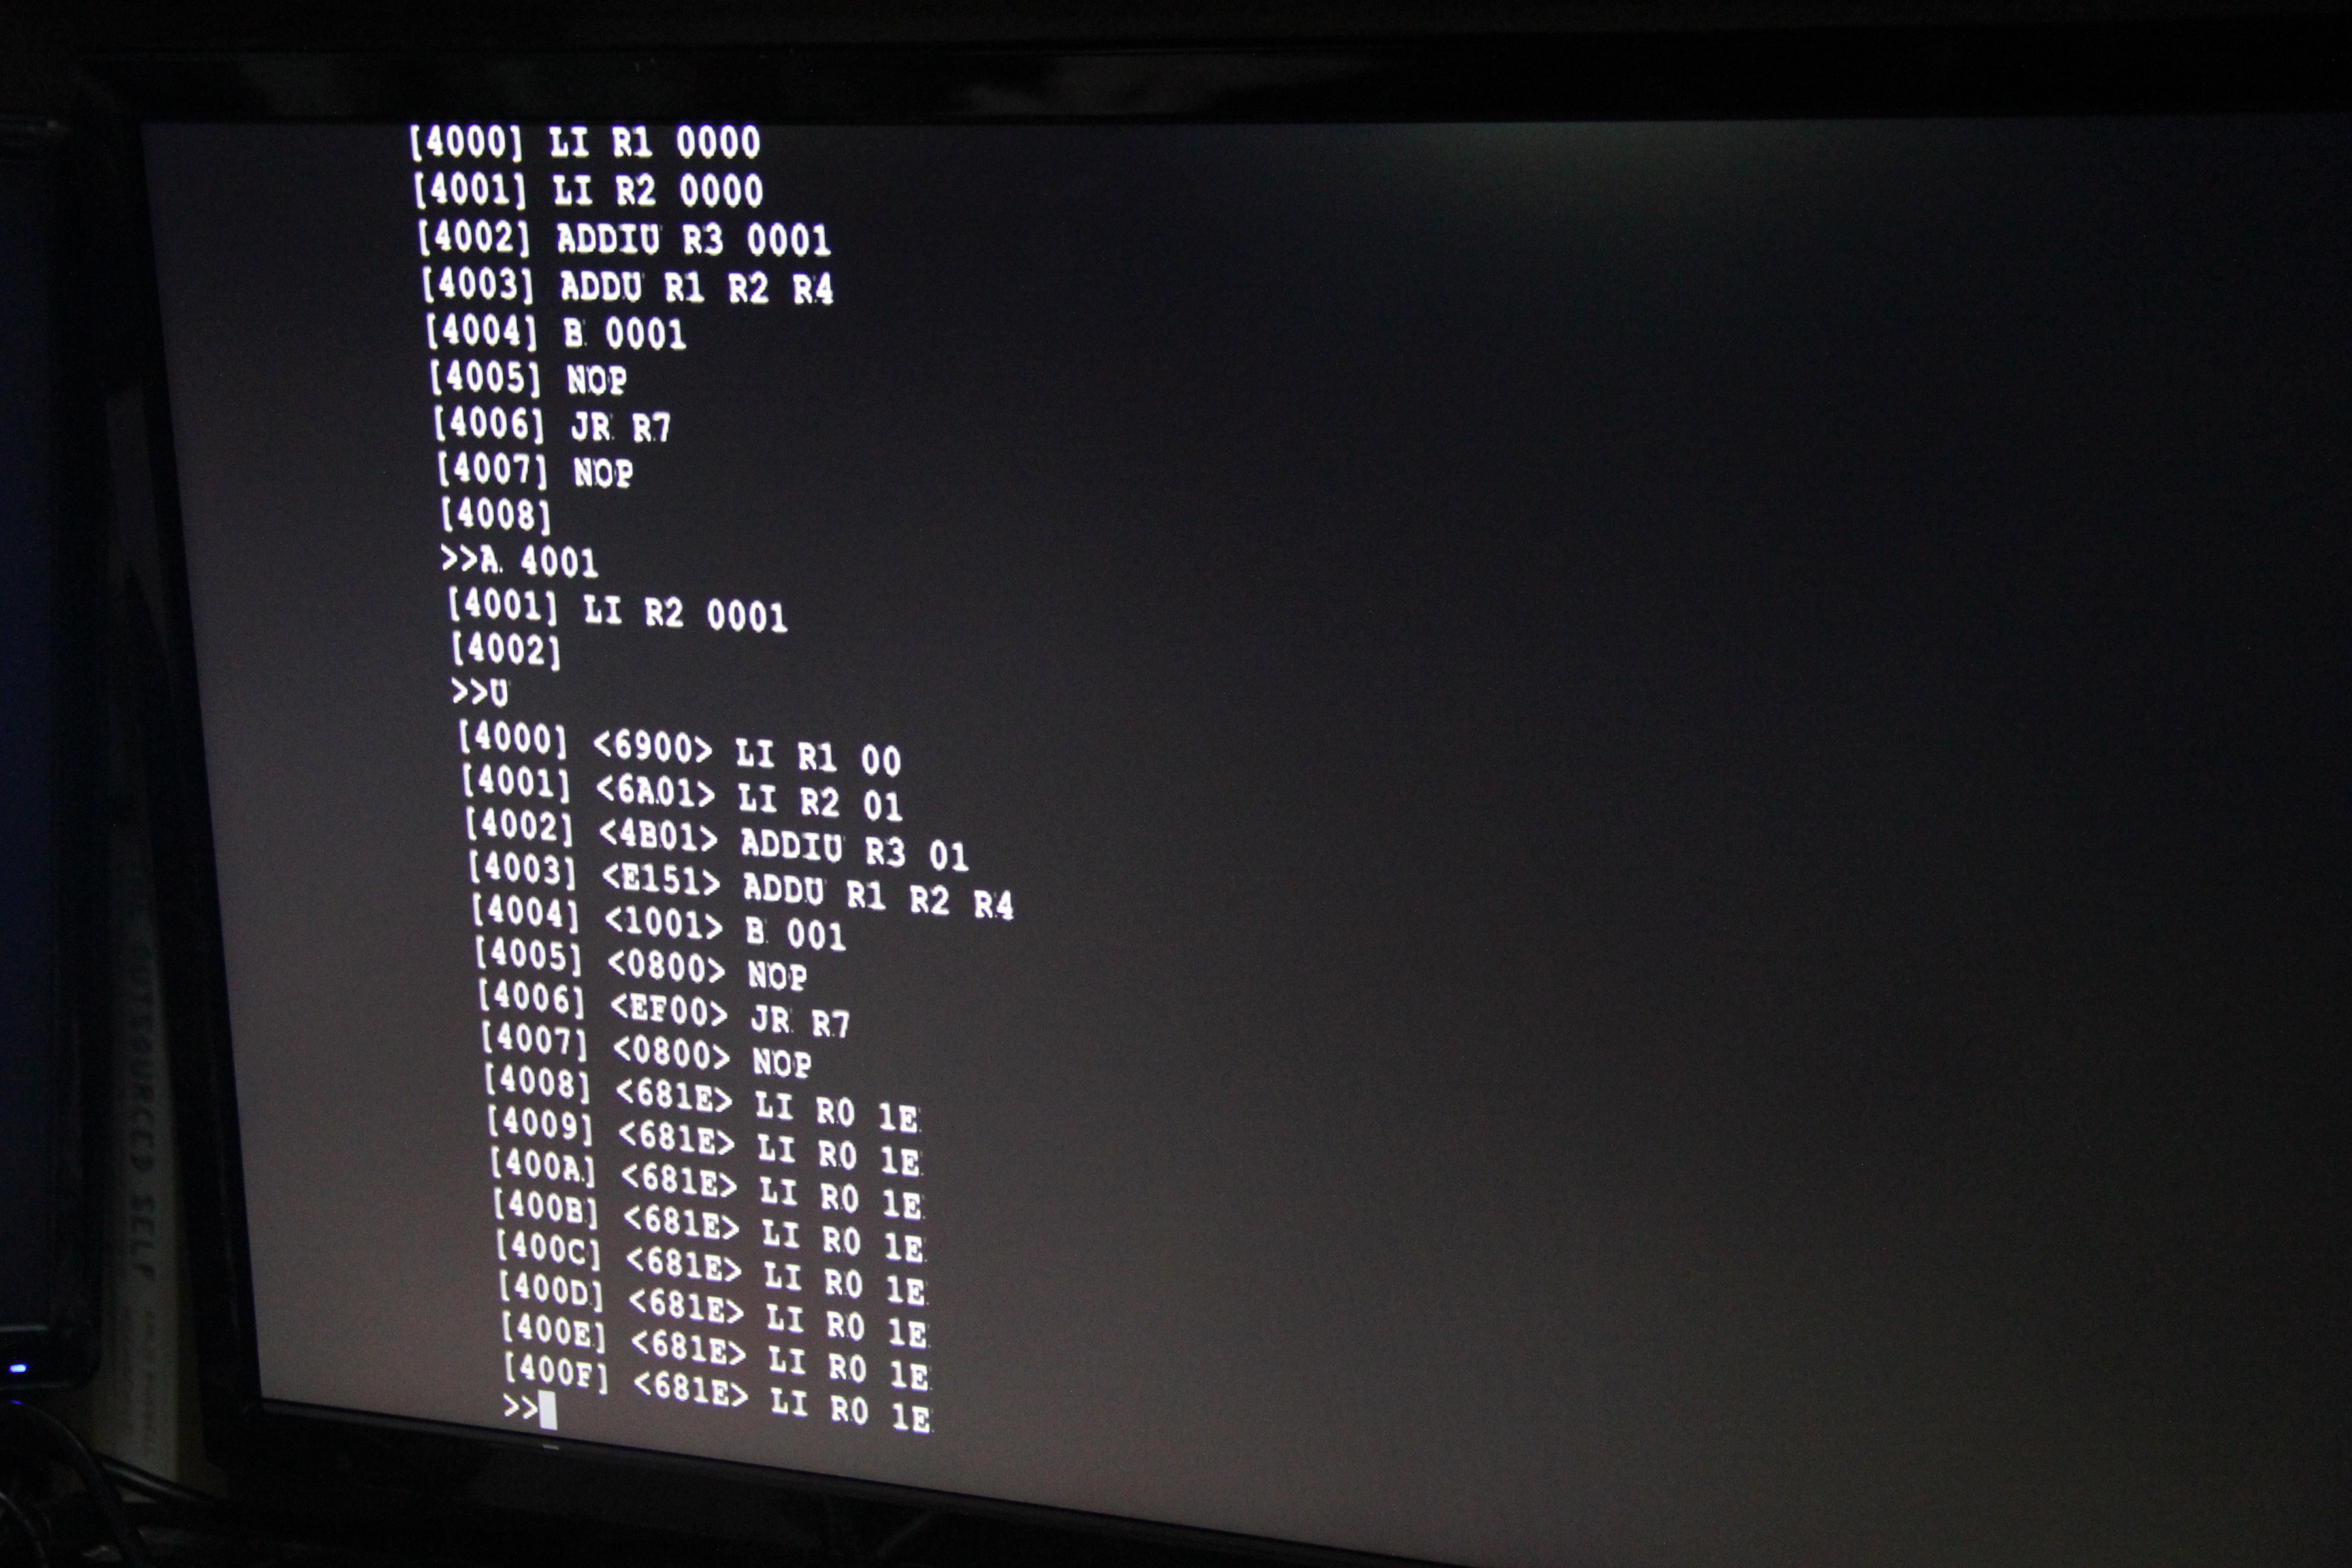
\includegraphics[width=4.5in]{Figures/picture/IMG_7236.JPG}
  \caption{U指令}
\end{figure}

可以看到,指令已经被正确地写入了。此时,我们输入斐波那契数列计算的汇编码,并运行,通过D指令查看内存的值以显示结果是否正确。

\begin{figure}[H]
  \centering
  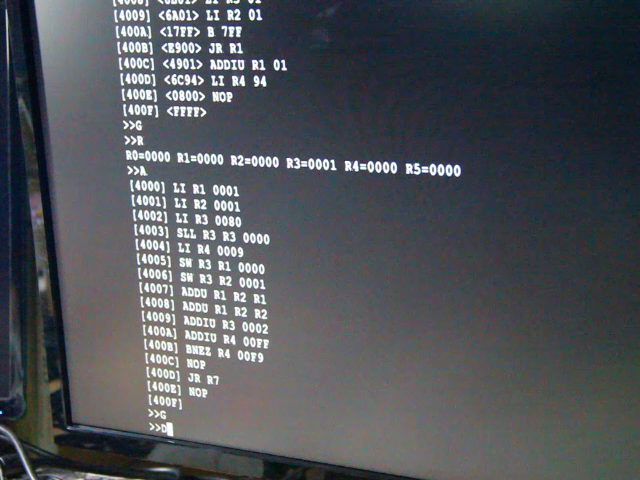
\includegraphics[width=4.5in]{Figures/picture/vlcsnap-2015-12-09-23h47m55s801.png}
  \caption{G指令}
\end{figure}

\begin{figure}[H]
  \centering
  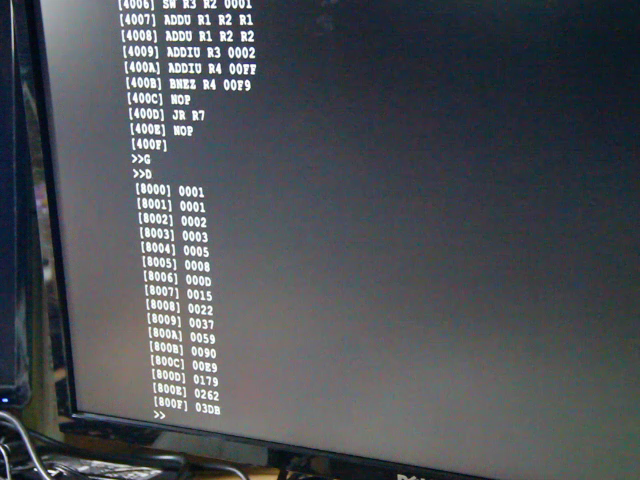
\includegraphics[width=4.5in]{Figures/picture/vlcsnap-2015-12-09-23h48m01s993.png}
  \caption{D指令}
\end{figure}

以上D指令内存的值表示斐波那契数列被正确地计算。最后,我们演示一下Control C中断。通过写入一个死循环程序,G指令运行,通过Ctrl-C组合键退出,并输出中断信息。

\begin{figure}[H]
  \centering
  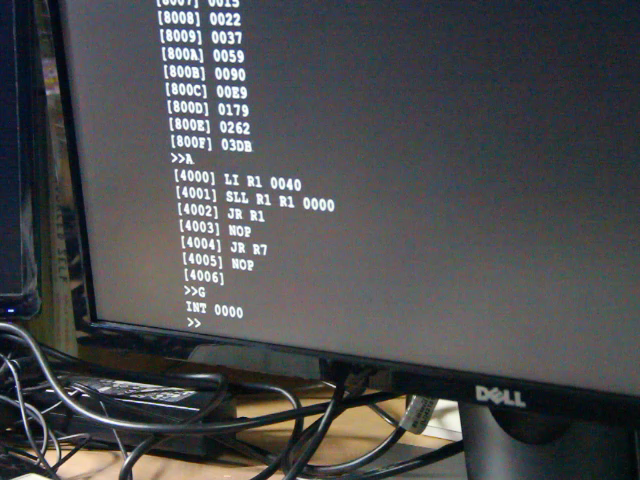
\includegraphics[width=4.5in]{Figures/picture/vlcsnap-2015-12-09-23h48m27s710.png}
  \caption{D指令}
\end{figure}



%----------------------------------------------------------------------------------------
%	SECTION 3
%----------------------------------------------------------------------------------------

\section{多道程序}

在多道程序的CPU,我们同时运行两套监控程序,一个为电脑端term程序,另一个为键盘VGA显示term程序。两套程序均可正确运行。

程序烧入后,可以看到电脑与VGA上均显示出OK。

\begin{figure}[H]
  \centering
  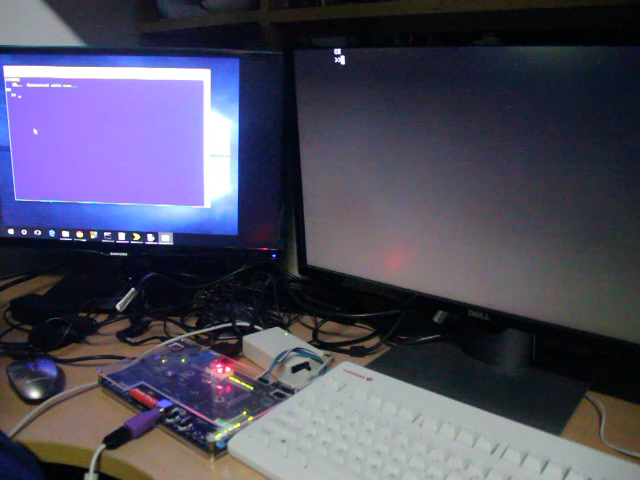
\includegraphics[width=4.5in]{Figures/picture/vlcsnap-2015-12-10-00h17m16s488.png}
  \caption{多道程序初始化}
\end{figure}

我们在电脑term终端输入几条指令到0x4000地址,并通过键盘VGA版的U指令查看写入的指令是否正确。

\begin{figure}[H]
  \centering
  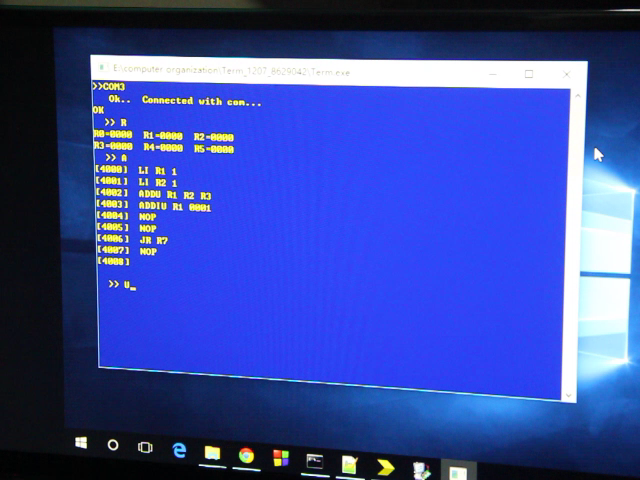
\includegraphics[width=4.5in]{Figures/picture/vlcsnap-2015-12-10-00h17m47s086.png}
  \caption{电脑端A、U指令}
\end{figure}

\begin{figure}[H]
  \centering
  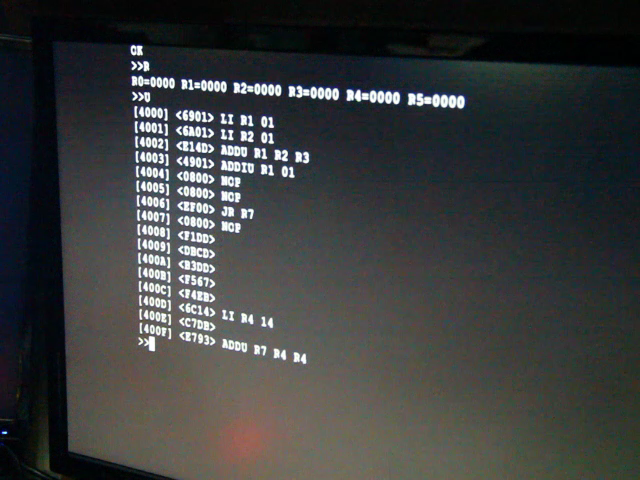
\includegraphics[width=4.5in]{Figures/picture/vlcsnap-2015-12-10-00h18m07s281.png}
  \caption{VGA端U指令}
\end{figure}

在键盘VGA版term程序中通过A指令更改某一条指令,并通过电脑端term查看更改是否正确。

\begin{figure}[H]
  \centering
  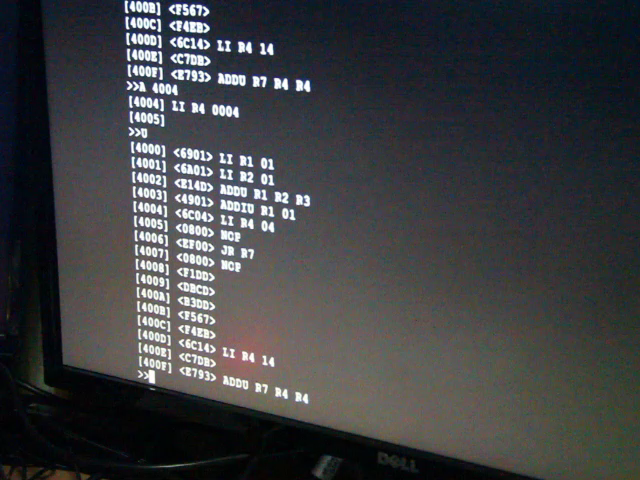
\includegraphics[width=4.5in]{Figures/picture/vlcsnap-2015-12-10-00h18m33s048.png}
  \caption{VGA端A、U指令}
\end{figure}

\begin{figure}[H]
  \centering
  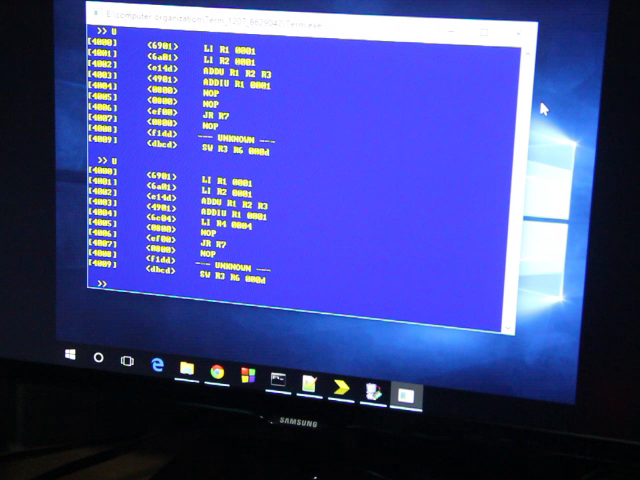
\includegraphics[width=4.5in]{Figures/picture/vlcsnap-2015-12-10-00h18m41s120.png}
  \caption{电脑端U指令}
\end{figure}

电脑端term运行指令,通过R查看寄存器的值是否改变。

\begin{figure}[H]
  \centering
  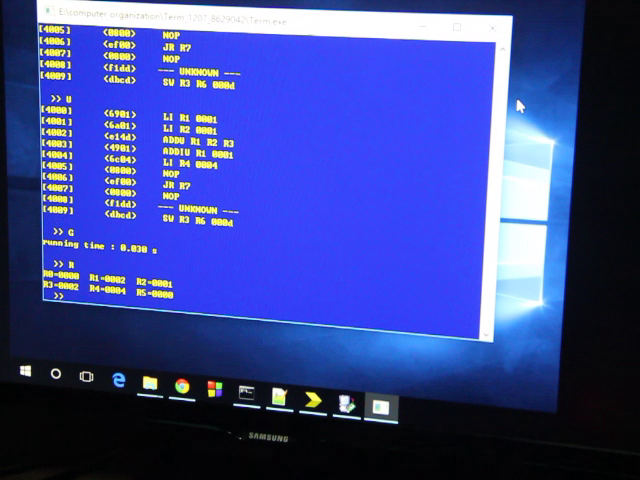
\includegraphics[width=4.5in]{Figures/picture/vlcsnap-2015-12-10-00h19m17s659.png}
  \caption{电脑端R指令}
\end{figure}

在VGA终端查看寄存器的值,发现没有改变,说明两套监控程序的寄存器相互独立。然后运行之前的指令,再次查看寄存器值,发现变为了与电脑端一样。

\begin{figure}[H]
  \centering
  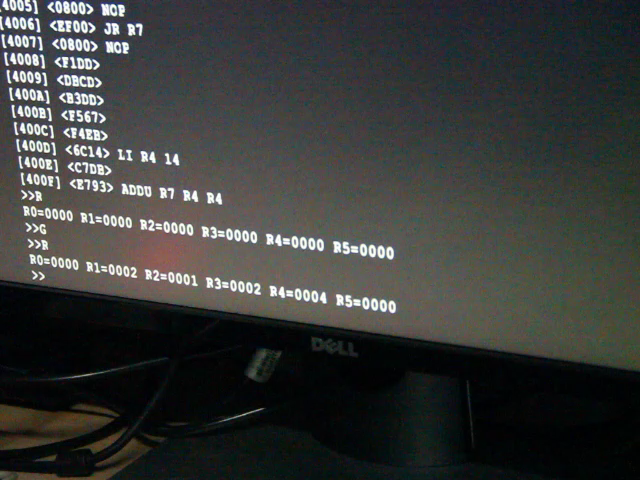
\includegraphics[width=4.5in]{Figures/picture/vlcsnap-2015-12-10-00h19m57s104.png}
  \caption{VGA端R指令}
\end{figure}

以上的演示说明了我们多道程序的正常工作,同时两套监控程序完全独立,也展示出了我们编写CPU作业的亮点。


 


%----------------------------------------------------------------------------------------
%	BIBLIOGRAPHY
%----------------------------------------------------------------------------------------

\printbibliography[heading=bibintoc]

%----------------------------------------------------------------------------------------

\end{document} 